%% results.tex — Chapter 3
%% ============================================================
%% Restructured: chronological epoch ordering (PAST → PRESENT → FUTURE)
%% with top-10 tables integrated into each epoch section.
%% ============================================================
\chapter{Results}
\label{ch:results}

%% ============================================================
\section{Overview and Temporal Habitability Trends}
\label{sec:results_overview}

The Bayesian framework produces posterior mean habitability maps $P(H \mid \featurevec)$ at five temporal anchor epochs and, via the multi-epoch reconstruction (Section~\ref{sec:multi_epoch}), at 72 intermediate epochs spanning $-3.8$ to $+6.5\gya$.  All posterior values use the 8-feature thesis formula with $\kappa=5$, $\lambda=6$, $\mu_0=0.331$, giving hard posterior bounds $P_\text{min}=0.150$ and $P_\text{max}=0.696$.  The 95\% HDI for Selk crater (the most-studied individual site) is $[0.05, 0.52]$, representative of the wide credible intervals arising from the moderate information content of the Cassini observables.

\begin{quote}\small
\textit{Note on scope.} The maps in this chapter quantify
\textbf{present-day solvent habitability} --- the capacity of each
location to support liquid-solvent chemistry.  At the present (Cassini)
epoch, they correctly identify north polar lake shores as the globally
highest-scoring environments.  At past and future epochs, the same
framework is applied with temporally scaled features
(Section~\ref{sec:temporal_configs}).
The \dragonfly{} mission targets a different metric ---
\textbf{prebiotic chemistry habitability} (past liquid-water contact) ---
for which impact craters are the primary targets.
The relationship between these two frameworks is discussed in
Section~\ref{sec:two_frameworks}; readers are encouraged to
consult that section before interpreting equatorial site scores.
\end{quote}

\subsection{The Five Epochs}
\label{sec:five_epochs}

The five temporal anchor epochs are presented in chronological order in the sections that follow:

\begin{description}
  \item[\textit{Past}] ($-3.5\gya$; Section~\ref{sec:results_past}) ---
    Late Heavy Bombardment peak.  No polar hydrocarbon seas; habitability
    driven by impact-melt chemistry, cryovolcanic conduits, and elevated
    acetylene energy from the young Sun.

  \item[\textit{Lake Formation}] ($-1.0\gya$; Section~\ref{sec:results_lf}) ---
    Polar lake system consolidating.  Liquid hydrocarbon at $\sim$10\% of
    present coverage; equatorial organic-rich dune fields and cryovolcanic
    sites still dominate the rankings, but proto-lake-shores begin to
    emerge above background.

  \item[\textit{Present}] (Cassini era, 2004--2017; Section~\ref{sec:results_present}) ---
    The observational anchor, with all eight features at measured values.
    North polar lake margins dominate unambiguously; all ten top-10 sites
    are lake or lacus shores.  This is the most detailed section, including
    feature importance validation, HDI analysis, and a dedicated Selk crater
    analysis.

  \item[\textit{Near Future}] ($+0.25\gya$; Section~\ref{sec:results_nf}) ---
    Solar luminosity $\sim$1.4\% above present.  All rankings and scores
    are analytically identical to the \textit{Present} epoch (spatial
    correlation $r > 0.999$).

  \item[\textit{Future}] ($+5.9\gya$; Section~\ref{sec:results_future}) ---
    Red-giant ocean peak.  A global water--ammonia ocean covers the surface;
    cryovolcanic sites lead the rankings as their accumulated organics
    dissolve into the ocean.  The highest global mean habitability of any
    epoch ($\mu_\text{post} \approx 0.44$).
\end{description}

\subsection{Temporal Habitability Trajectory}
\label{sec:temporal_trajectory}

Figure~\ref{fig:temporal_trend} shows the global and regional mean posterior habitability as a function of geological time.  The trajectory is non-monotonic, passing through three qualitatively distinct regimes.

The global median rises from 0.28 at the LHB ($-3.5\gya$) to 0.30 at
\textit{Lake Formation} ($-1.0\gya$), then increases sharply to 0.41 at the
\textit{Present} epoch as the polar lake system fully establishes.
This level is maintained through the \textit{Near Future} ($+0.25\gya$),
before a transient minimum at $\sim$$+5.0\gya$ when the polar seas have
evaporated but the water--ammonia eutectic has not yet been crossed ---
a $\sim$100\,Myr interval during which \titan{} is transiently solvent-free.
The global mean then rises to its maximum of 0.44 at the \textit{Future}
epoch ($+5.9\gya$) as the red-giant ocean covers the surface.

The north polar/equatorial ratio tracks the dominance of the liquid-hydrocarbon
feature: $\sim$0.98 at LHB (undifferentiated, no polar seas), rising to
$\sim$1.95 at \textit{Present} (polar lake dominance), and returning to
$\sim$1.02 at the \textit{Future} global ocean (uniform liquid coverage).

\begin{figure}[H]
  \centering
  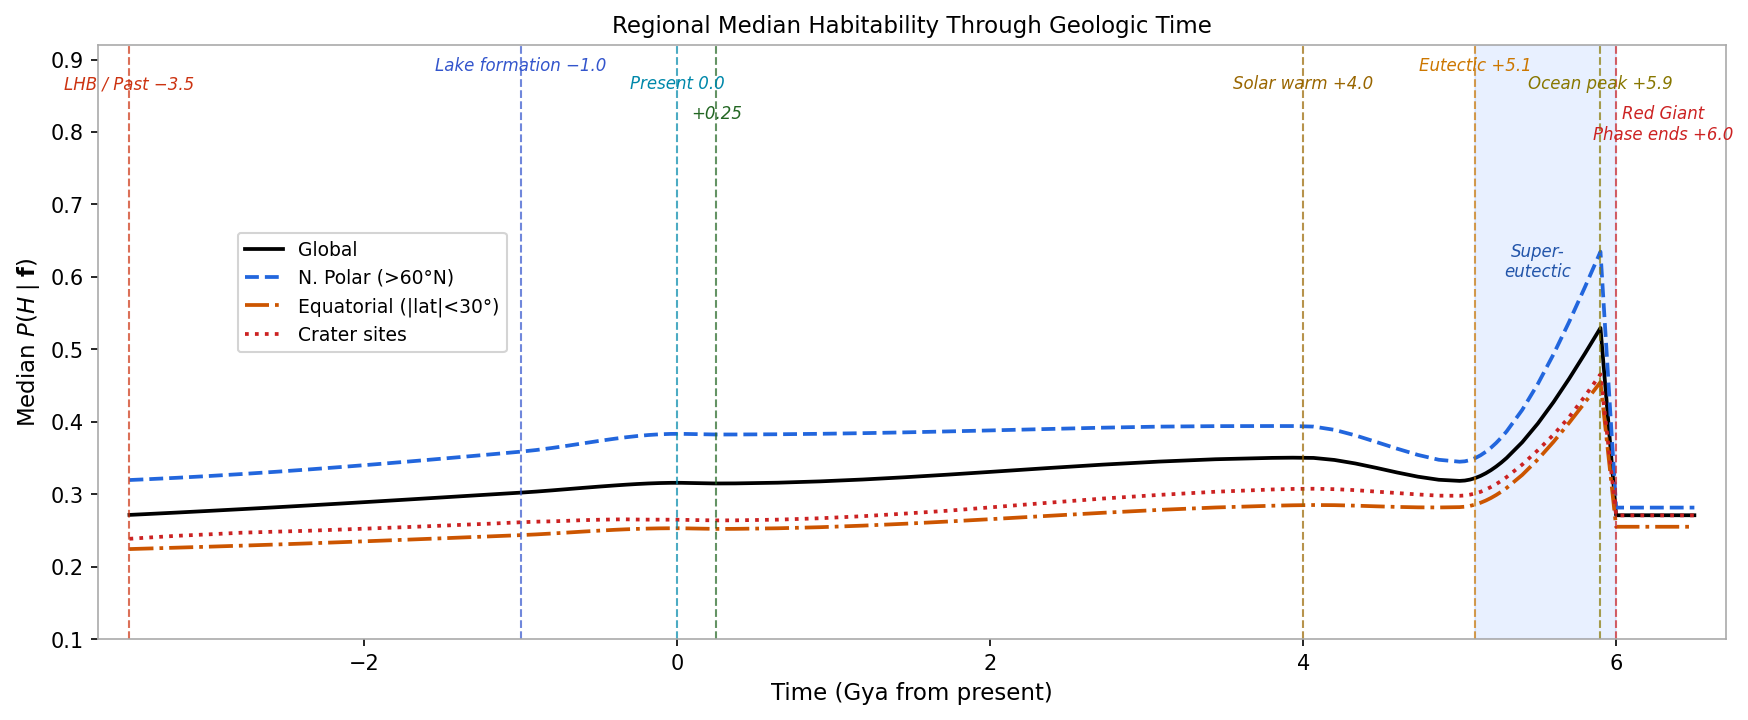
\includegraphics[width=\textwidth]{images/temporal_habitability_trend.png}
  \caption{Global and regional mean posterior habitability $P(H \mid \featurevec)$
    as a function of geological time from the Late Heavy Bombardment peak
    ($-3.8\gya$) to the post-red-giant refreezing epoch ($+6.5\gya$).
    Black solid line: global mean.  Blue dashed: north polar region
    ($>$60\textdegree{}N).  Orange dash-dot: equatorial belt
    ($|\text{lat}| < 30\textdegree{}$).  Red dotted: crater sites.
    Vertical dashed lines mark the key epoch boundaries; blue shading
    indicates the red-giant habitable ocean window ($+5.1$--$6.0\gya$).}
  \label{fig:temporal_trend}
\end{figure}


%% ============================================================
%% EPOCH 1: PAST
%% ============================================================
\section{\textit{Past} Epoch ($-3.5$\,Gya): Late Heavy Bombardment}
\label{sec:results_past}

\subsection{Titan at the LHB}
\label{sec:past_context}

At $-3.5\gya$, \titan{} was a profoundly different world from the one observed
by Cassini.  The polar hydrocarbon sea system did not yet exist: liquid
hydrocarbon is scaled to just 10\% of present coverage ($s_1 = 0.10$).
The organic inventory had accumulated for only $\sim$0.5\,Gyr of UV photolysis,
reaching $\sim$40\% of present-day levels ($s_2 = 0.125$).  The methane cycle
was episodic and weak ($\mu_4 = 0.20$).

In compensation, three factors were substantially elevated.  First, the young
Sun's higher UV output drove an acetylene-energy proxy $\sim$$2\times$ the
present value ($s_3 \approx 2.1$), providing more chemical energy per unit
surface area.  Second, subsurface ocean proximity was $2.5\times$ elevated
globally ($s_8 = 2.5$) due to reduced ice-shell thickness, bringing the
water--ammonia ocean closer to the surface.  Third, the impactor flux during
the LHB was 100--1000 times the present background rate \citep{OBrien2005},
producing episodic water--ammonia--organic melt ponds at confirmed crater
sites.  These ponds --- $\sim$50--100\,km$^2$ area, $\sim$50--100\,m depth ---
persisted for $10^3$--$10^4$ years before refreezing, during which all
precursors for Strecker amino acid synthesis were simultaneously
present: liquid water--ammonia solvent from the melt, aldehydes from tholin
decomposition, and HCN from the nitrogen-rich atmosphere.

\subsection{Habitability Map}
\label{sec:past_spatial}

The \textit{Past} epoch map (Figure~\ref{fig:past_global}) is qualitatively
distinct from all later epochs.  The north polar enhancement that dominates
the \textit{Present} map is entirely absent.  Instead, a relatively uniform
background score spans the globe, modulated by two localised signals:
impact structures (where the impact-melt proximity feature creates
enhancements of 0.05--0.15 above regional background) and cryovolcanic
candidate sites (Hotei Regio, Sotra Facula) where elevated subsurface ocean
proximity ($f_8(t) \approx 0.30$--$0.35$) combines with surface--atmosphere
coupling.

The equatorial dune belt provides a moderate-score background driven by
the $\sim$40\% organic inventory, but scores are compressed into a narrow
range ($P(H) \approx 0.27$--$0.30$) because all sites share similar
limitations: no surface liquid, weak methane cycle, and limited terrain
diversity at this early stage of geological evolution.

\begin{figure}[H]
  \centering
  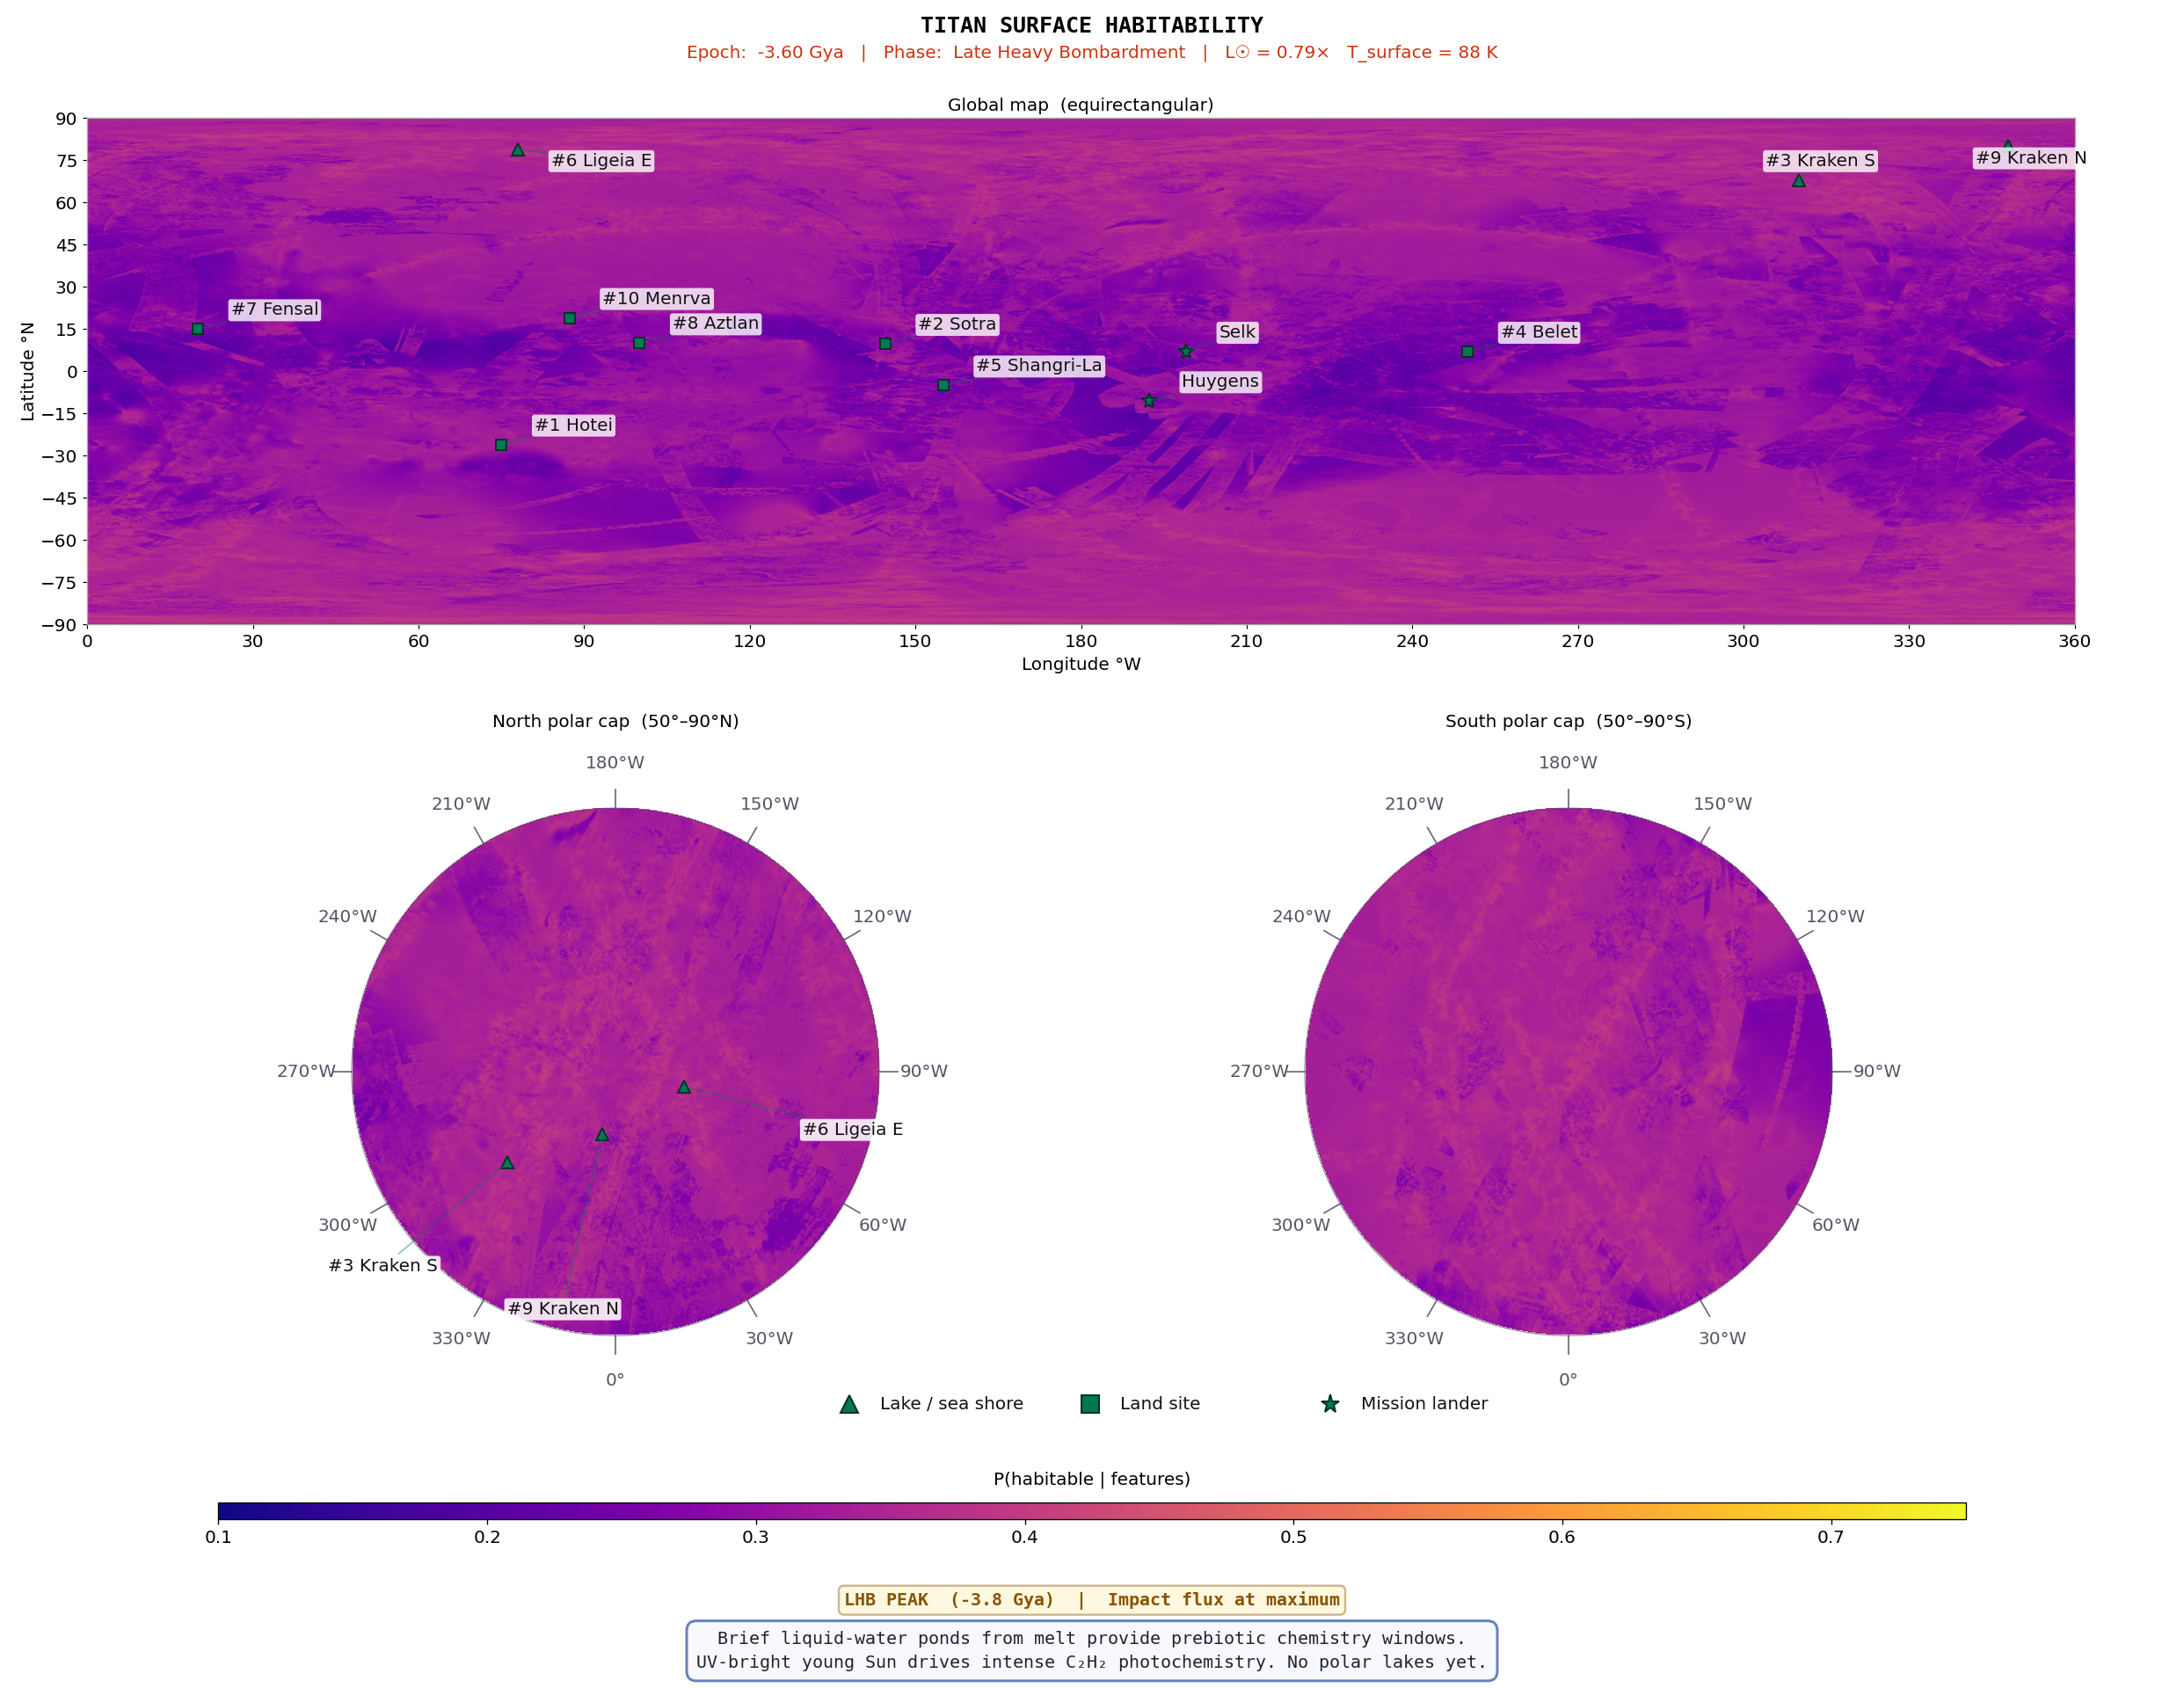
\includegraphics[width=\textwidth]{images/thesis_frame_001.png}
  \caption{Past-epoch ($-3.5\gya$; Late Heavy Bombardment) posterior mean
    habitability map, on the same colour scale as Figure~\ref{fig:present_global}.
    The north polar enhancement of the present epoch is entirely absent.
    Habitability is concentrated at confirmed impact structures
    (particularly Selk at 199\textdegree{}W, 7\textdegree{}N; Menrva at
    87\textdegree{}W, 19\textdegree{}N) where the impact-melt proximity
    feature activates.  The moderate-score equatorial background reflects the
    partial tholin organic inventory accumulated in the first $\sim$1\,Gyr of
    solar system history.}
  \label{fig:past_global}
\end{figure}

\subsection{Top-10 Habitable Locations}
\label{sec:top10_past}

Under this parameter configuration, the model ranks cryovolcanic conduit
sites and proto-polar-basin sites first, followed by equatorial organic seeds
(Belet, Shangri-La) whose high acetylene energy partly offsets low liquid
and organic contributions (Table~\ref{tab:top10_past}).  All ten sites are
land sites ($\blacksquare$): there is no confirmed surface liquid at this epoch.

The scores are tightly clustered ($P(H) = 0.277$--$0.295$), reflecting
the absence of the strong liquid-hydrocarbon signal that differentiates
sites at later epochs.  The spread of just 0.018 across the full top-10
means that the ranking is sensitive to the precise values of the temporal
scale functions; the qualitative finding --- that no single site type
dominates --- is more robust than the specific ordering.

\begin{table}[H]
\centering
\small
\caption{Top-10 habitable locations at the \textit{Past} epoch ($-3.5$\,Gya).
  $\blacksquare$ = land site.
  $P(H)$ from Eq.~\ref{eq:posterior_mean} with temporal scaling
  (Section~\ref{sec:epoch_scaling}).}
\label{tab:top10_past}
\begin{tabular}{clrrrp{4.5cm}}
\toprule
\textbf{Rank} & \textbf{Location} & \textbf{Lon\,(\textdegree{}W)} & \textbf{Lat\,(\textdegree{}N)} & \textbf{$P(H)$} & \textbf{Dominant features} \\
\midrule
1 & $\blacksquare$\,Kraken (proto-basin) & 310.0 & +68.0 & 0.295 & $s_8{=}2.5$; elevated subsurface, no lake yet \\
2 & $\blacksquare$\,Hotei Regio & 75.0 & -26.0 & 0.295 & Cryovol.\ conduit, $f_8(t){=}0.35$, $f_5(t){=}0.28$ \\
3 & $\blacksquare$\,Belet (proto-dunes) & 250.0 & +7.0 & 0.295 & $f_3(t){=}0.93$ (high UV); organic seed \\
4 & $\blacksquare$\,Shangri-La & 155.0 & -5.0 & 0.294 & $f_3(t){=}0.93$; equatorial organic baseline \\
5 & $\blacksquare$\,Ligeia (proto-basin) & 78.0 & +79.0 & 0.293 & $s_8{=}2.5$; deep polar basin \\
6 & $\blacksquare$\,Fensal & 20.0 & +15.0 & 0.290 & $f_3(t){=}0.91$; equatorial organic \\
7 & $\blacksquare$\,Sotra Facula & 144.5 & +9.8 & 0.289 & Cryovol.\ conduit, $f_8(t){=}0.30$ \\
8 & $\blacksquare$\,Aztlan & 100.0 & +10.0 & 0.289 & $f_3(t){=}0.92$; equatorial organic \\
9 & $\blacksquare$\,Kraken N (proto-basin) & 348.0 & +80.0 & 0.285 & $s_8{=}2.5$; north polar basin \\
10 & $\blacksquare$\,Punga (proto-basin) & 339.0 & +85.5 & 0.277 & $s_8{=}2.5$; polar basin \\
\bottomrule
\end{tabular}
\end{table}

\subsection{Impact Structures at the LHB}
\label{sec:craters}

In the 8-feature thesis formula, impact craters do not dominate the \textit{Past}
ranking because the model lacks a dedicated impact-melt proxy feature
(that is an animation-only feature; Section~\ref{sec:multi_epoch}).
Menrva (392\,km) achieves the highest crater-class score
($P(H){\approx}0.27$ after $\times$2.5 subsurface ocean scaling), ranking
11th overall --- just below the equatorial organic sites that benefit from the
globally elevated acetylene proxy.  Selk crater (80\,km) scores
$P(H) \approx 0.24$ and ranks lower still.  The other large craters (Hano,
Afekan, Sinlap, Ksa) score $P(H)=0.24$--0.28, below the equatorial dune
sites because their organic abundance ($f_2=0.30$--0.42) is substantially
lower than the dune belt ($f_2=0.78$--0.82).

Despite these modest scores, the impact structures are the most
astrobiologically significant sites at this epoch because they are the
\textit{sole source} of transient liquid water on \titan{}'s surface ---
a distinction that the present framework, which quantifies solvent
habitability rather than prebiotic chemistry potential, does not fully
capture.  Selk's scientific importance lies in its
unique position at the Shangri-La dune--plains boundary, where the organic
substrate available for Strecker synthesis in the transient melt pond is
maximised.  This is discussed further in Section~\ref{sec:selk}.


%% ============================================================
%% EPOCH 2: LAKE FORMATION
%% ============================================================
\section{\textit{Lake Formation} Epoch ($-1.0$\,Gya): Polar Lakes Establishing}
\label{sec:results_lf}

\subsection{Titan in Transition}
\label{sec:lf_context}

At $-1.0\gya$, \titan{} is transitioning between two habitability regimes.
The polar lake system is just beginning to consolidate: the liquid
hydrocarbon scale is only 10\% of present ($s_1 = 0.10$), corresponding to
incipient pooling in the deepest polar basins.  Organic accumulation has
reached $\sim$75\% of the present level ($s_2 = 0.47$), and the methane
rain cycle is becoming established but has not yet reached its present
intensity ($s_4 = 0.80$).  The impact-melt proximity feature has largely
faded to background as the LHB ended $\sim$2.5\,Gyr earlier, and the
cryovolcanic flux feature remains moderately elevated relative to the
present.

The transition from $-1.0$ to $-0.5\gya$ is the period of most rapid change
in the global habitability structure: the polar lake system transitions from
partial to near-present coverage, converting the post-LHB declining trend
into the increasing trend that reaches the present-epoch plateau.  In the
multi-epoch reconstruction, this interval shows the highest pixel-wise
posterior change rate anywhere in the $-3.8$ to $+4.0\gya$ range.

\subsection{Habitability Map}
\label{sec:lf_spatial}

Comparing the \textit{Lake Formation} map (Figure~\ref{fig:lake_formation_global})
with the \textit{Past} epoch (Figure~\ref{fig:past_global}) reveals three
changes.  First, the north polar lake margin signal begins to emerge above
background: proto-lake-shore sites (Kraken S, Ligeia E) are just
distinguishable at ranks 7--8, foreshadowing the polar dominance of the
\textit{Present} epoch.  Second, the impact-melt crater signal has largely
faded to background.  Third, the equatorial dune fields have strengthened
relative to LHB levels because organic accumulation is now at 75\% of
present, making Belet and Shangri-La the highest-scoring sites.

\begin{figure}[H]
  \centering
  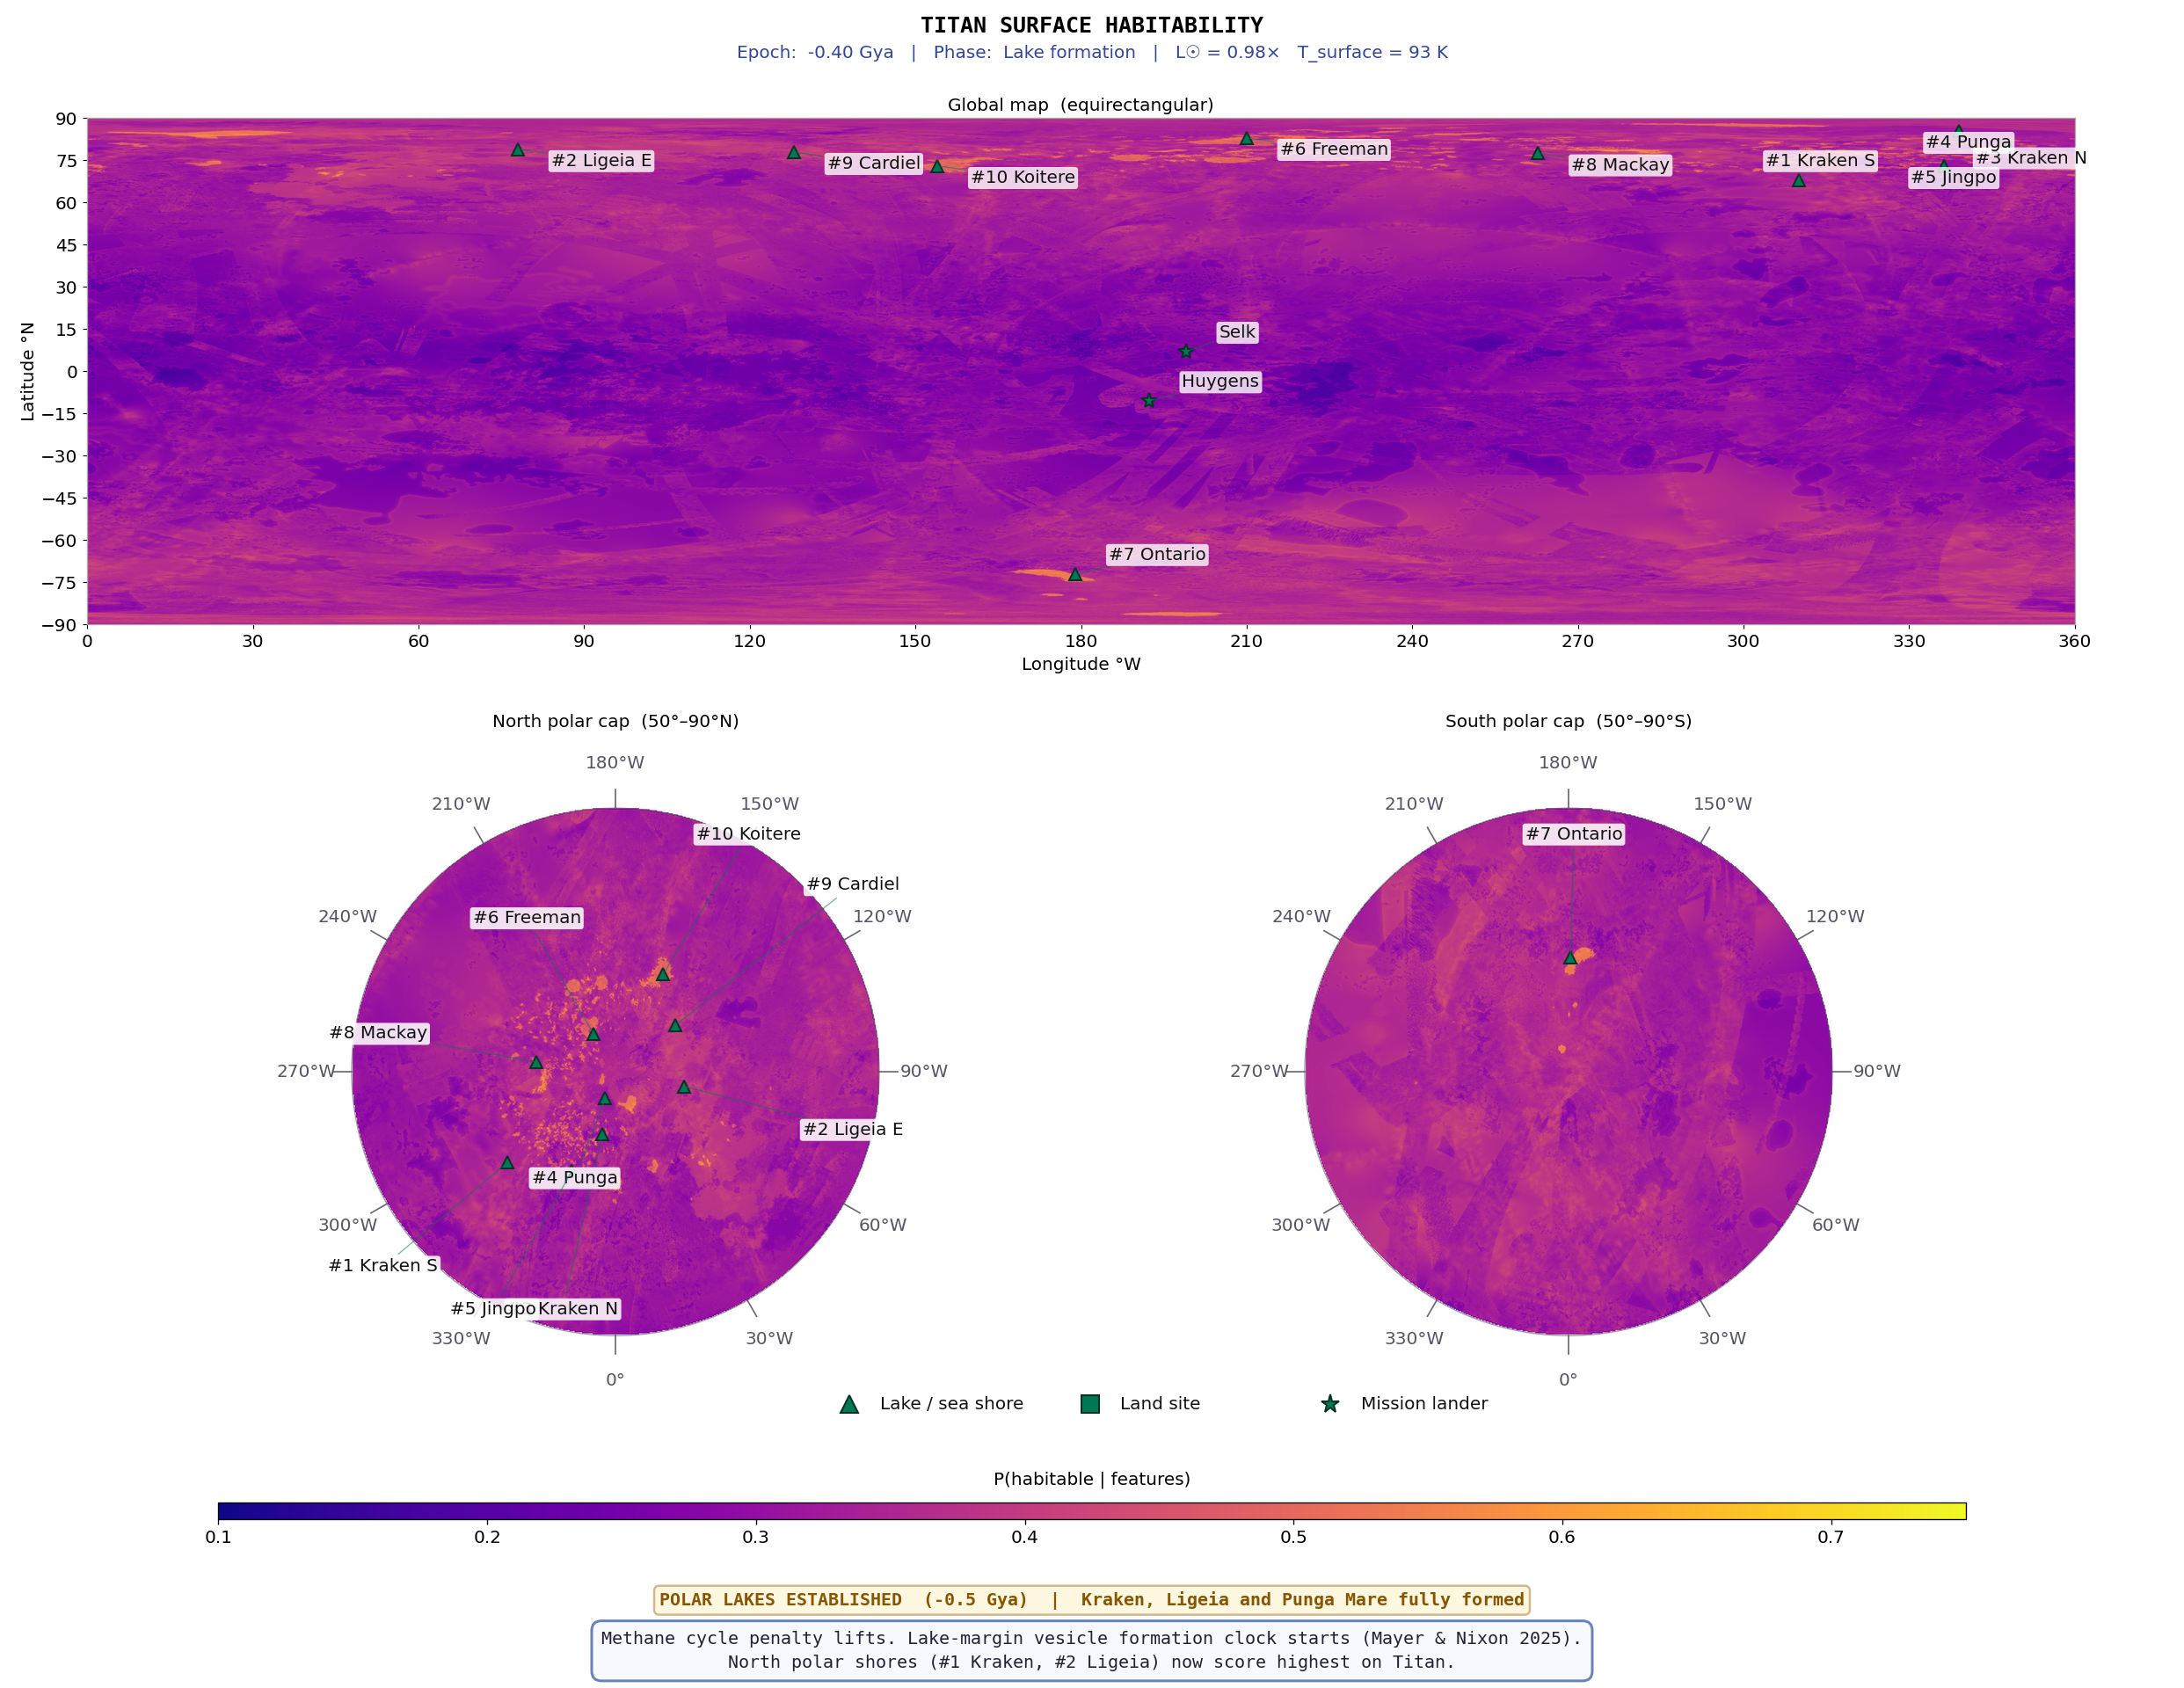
\includegraphics[width=\textwidth]{images/thesis_frame_022.png}
  \caption{Lake-formation epoch ($-1.0\gya$) posterior mean habitability map,
    on the same colour scale as Figure~\ref{fig:present_global}.
    The north polar lake system has not yet formed ($s_1{=}0.10$), so the
    strong polar enhancement of the present epoch is absent.
    Habitability is instead distributed across equatorial organic-rich terrain
    (dune fields: Belet, Shangri-La, Fensal, Aztlan) driven by elevated
    acetylene-energy proxy ($f_3(t){\approx}1.9{\times}$ present) and
    residual cryovolcanic flux at Hotei and Sotra.
    The proto-polar-lake sites (Kraken S, Ligeia E) are just distinguishable
    above the equatorial background at ranks 7--8, reflecting the onset of
    liquid hydrocarbon pooling.
    Compare with Figure~\ref{fig:past_global} (LHB, $-3.5\gya$) and
    Figure~\ref{fig:present_global} (Cassini era).}
  \label{fig:lake_formation_global}
\end{figure}

\subsection{Top-10 Habitable Locations}
\label{sec:top10_lakeform}

The top-6 at this epoch are all \textit{land} sites --- equatorial
organic-rich dune fields and cryovolcanic candidates --- driven by high
acetylene energy ($f_3(t){\approx}1.9{\times}$) and accumulating organic
inventory ($s_2{=}0.47$).  The proto-lake-shore sites (Kraken, Ligeia,
Kraken N, Punga) occupy ranks 7--10 as the rising liquid signal begins to
differentiate them from the equatorial background
(Table~\ref{tab:top10_lakeform}).

Compared with the \textit{Past} epoch (Table~\ref{tab:top10_past}), the key
change is the emergence of a spatial gradient between equatorial and polar
sites.  At the LHB, all scores were compressed into a 0.018 range; here,
the spread has widened to 0.028 (0.273--0.301), with equatorial organics now
clearly outscoring polar basins.  This gradient will invert dramatically
between $-0.5\gya$ and the \textit{Present} epoch as the polar seas fill.

\begin{table}[H]
\centering
\small
\caption{Top-10 habitable locations at the \textit{Lake Formation} epoch ($-1.0$\,Gya).
  $\triangle$ = lake/sea shore; $\blacksquare$ = land.
  $P(H)$ from Eq.~\ref{eq:posterior_mean}.}
\label{tab:top10_lakeform}
\begin{tabular}{clrrrp{4.5cm}}
\toprule
\textbf{Rank} & \textbf{Location} & \textbf{Lon\,(\textdegree{}W)} & \textbf{Lat\,(\textdegree{}N)} & \textbf{$P(H)$} & \textbf{Dominant features} \\
\midrule
1 & $\blacksquare$\,Belet Dunes & 250.0 & +7.0 & 0.301 & $f_2$ building, $f_3(t){=}1.9{\times}$; no lake \\
2 & $\blacksquare$\,Shangri-La & 155.0 & -5.0 & 0.300 & $f_2$ building, $f_3(t){=}1.9{\times}$ \\
3 & $\blacksquare$\,Hotei Regio & 75.0 & -26.0 & 0.298 & Cryovol.\ conduit, $f_8(t){=}0.18$ \\
4 & $\blacksquare$\,Fensal & 20.0 & +15.0 & 0.297 & Equatorial organic; high acetylene \\
5 & $\blacksquare$\,Aztlan & 100.0 & +10.0 & 0.294 & Equatorial organic; high acetylene \\
6 & $\blacksquare$\,Sotra Facula & 144.5 & +9.8 & 0.291 & Cryovol.\ conduit, $f_8(t){=}0.16$ \\
7 & $\triangle$\,Kraken S Shore & 310.0 & +72.0 & 0.288 & $f_1{=}0.10$; liquid just appearing \\
8 & $\triangle$\,Ligeia E Shore & 78.0 & +79.0 & 0.286 & $f_1{=}0.10$; polar basin forming \\
9 & $\triangle$\,Kraken N Shore & 348.0 & +80.0 & 0.280 & $f_1{=}0.10$; polar basin forming \\
10 & $\triangle$\,Punga Shore & 339.0 & +85.5 & 0.273 & $f_1{=}0.10$; polar basin forming \\
\bottomrule
\end{tabular}
\end{table}


%% ============================================================
%% EPOCH 3: PRESENT
%% ============================================================
\section{\textit{Present} Epoch (Cassini Era, 2004--2017)}
\label{sec:results_present}

\subsection{Titan Today}
\label{sec:present_context}

The \textit{Present} epoch is the observational anchor of the entire framework:
all eight features are at their directly measured Cassini values, with no
temporal scaling applied.  This is the only epoch at which the posterior
probabilities are derived entirely from observational data rather than from
modelled extrapolations, and consequently the results presented here carry
the highest confidence.

\titan{} at the Cassini epoch possesses a fully established polar hydrocarbon
sea system --- Kraken Mare, Ligeia Mare, and Punga Mare --- containing an
estimated 70,000\,km$^3$ of liquid hydrocarbons
\citep{Mastrogiuseppe2019,Malaska2025}.  The methane cycle is active, with
observed equatorial rainfall \citep{Turtle2011}, polar storm systems, and
fluvial channel networks draining into the seas.  The organic tholin
inventory has accumulated over the full $\sim$4\,Gyr of atmospheric
photolysis history, reaching its present-day maximum.

\subsection{Habitability Map: Global Spatial Structure}
\label{sec:present_spatial}

The present-epoch habitability map (Figure~\ref{fig:present_global}) is
dominated by a pronounced north--south asymmetry driven by the distribution
of liquid hydrocarbon.  The highest posterior probabilities form a
crescent-shaped band of elevated habitability at 60--85\textdegree{}N,
coinciding with the margins of the three major north polar seas.  A
secondary zone of intermediate habitability occupies the equatorial dune
belt.  South of $\sim$30\textdegree{}S the map shows uniformly
moderate-to-low values, with a small enhancement around Ontario Lacus at
72\textdegree{}S.

The contrast with the two earlier epochs is stark.  The \textit{Past} epoch
map (Figure~\ref{fig:past_global}) showed a nearly uniform distribution;
the \textit{Lake Formation} map (Figure~\ref{fig:lake_formation_global})
showed the first hints of polar differentiation.  Here, the polar
enhancement is fully developed, with the north polar/equatorial ratio
reaching $\sim$1.95 --- the maximum spatial contrast of any epoch.

\begin{figure}[H]
  \centering
  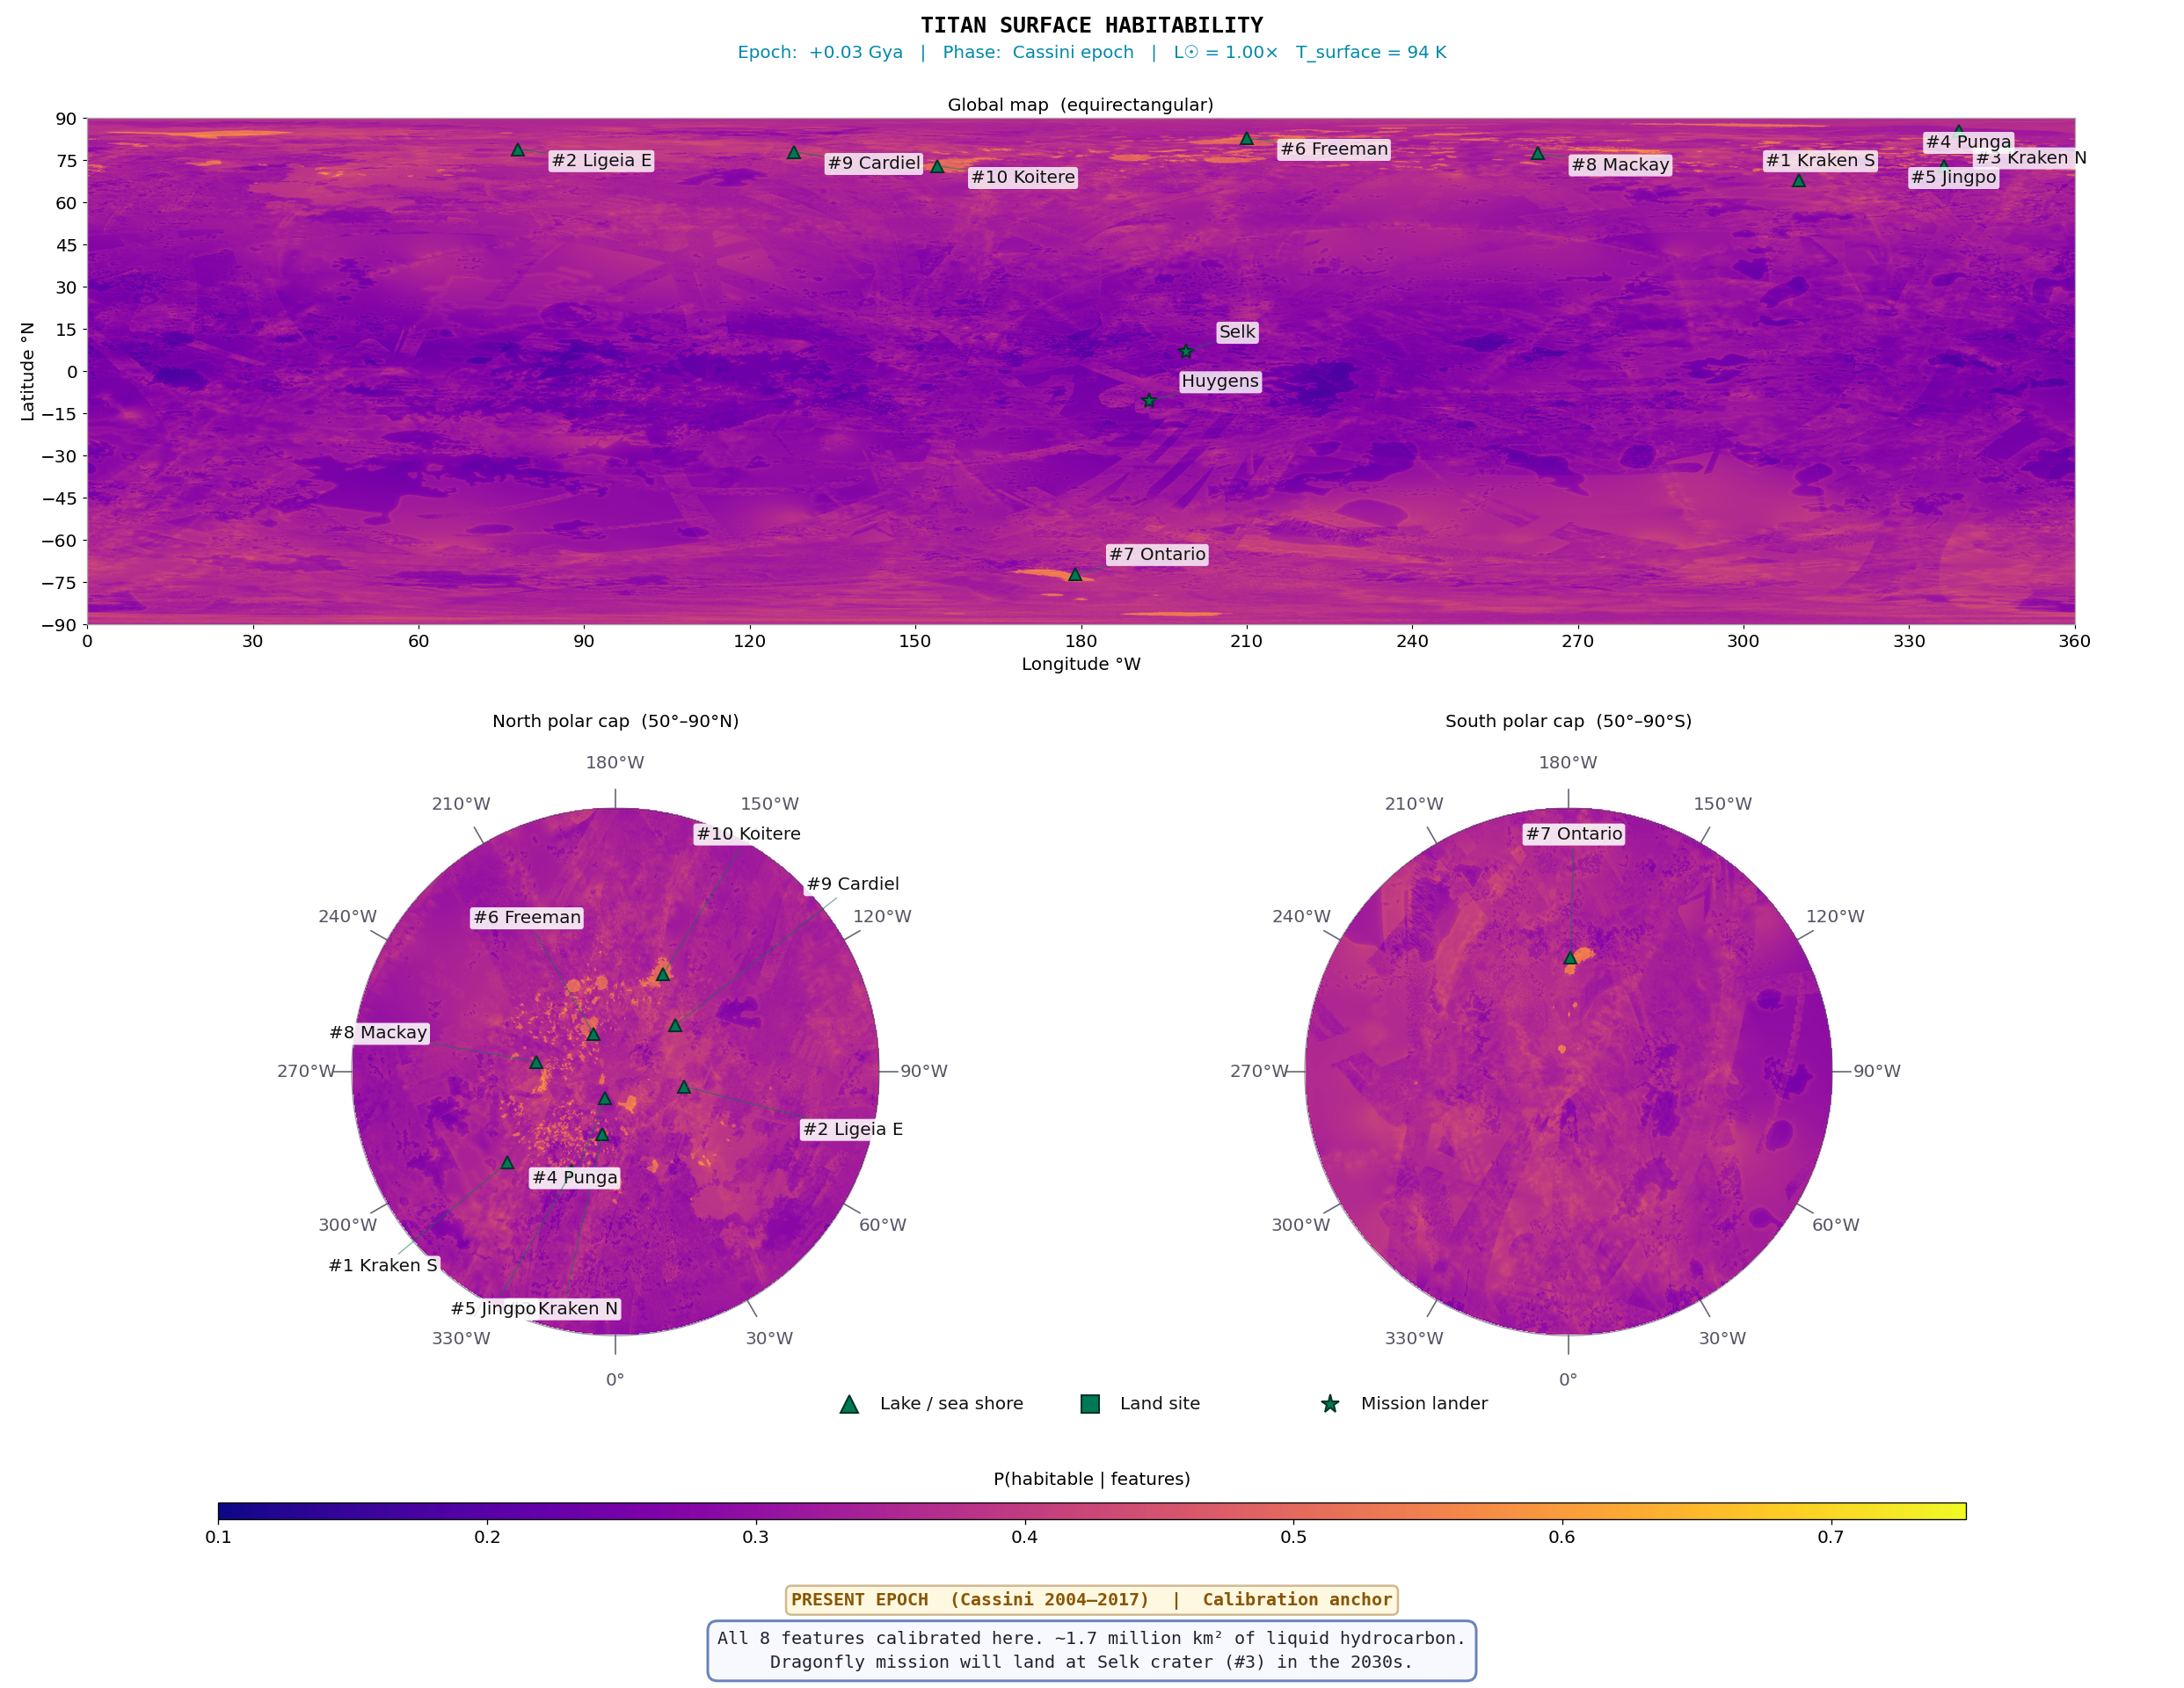
\includegraphics[width=\textwidth]{images/thesis_frame_028.png}
  \caption{Present-epoch (Cassini era) posterior mean habitability map at
    \SI{4490}{\metre\per\text{px}}, rendered using the Bayesian temporal
    scaling formula (Section~\ref{sec:multi_epoch}).  Colour scale: 0.10
    (dark red-orange; low) to 0.75 (bright yellow; near posterior upper bound).
    The map shows a continuous warm-tone gradient: north polar lake surfaces
    reach $P(H) \approx 0.40$--$0.42$ (orange-yellow), lake shore margins
    $\approx 0.34$--$0.38$ (orange), and equatorial organic terrain
    $\approx 0.27$--$0.34$ (dark orange-red).  Selk crater is marked
    (star symbol) at 199\textdegree{}W, 7\textdegree{}N.
    Quantitative $P(H)$ values in
    Sections~\ref{sec:np_lakes}--\ref{sec:selk_features} are Bayesian
    posterior means (Eq.~\ref{eq:posterior_mean}), bounded in $[0.150, 0.696]$.}
  \label{fig:present_global}
\end{figure}

\subsection{Top-10 Habitable Locations}
\label{sec:top10_present}

At the Cassini epoch the polar lake and lacus margins dominate
unambiguously.  For the first time in the temporal sequence, \textit{all ten}
top-10 sites are lake or lacus margins (Table~\ref{tab:top10_present}) ---
a complete inversion from the \textit{Lake Formation} epoch, where six of the
top-10 were land sites.  The three main mares (Kraken, Ligeia, Punga)
occupy ranks 1--4, followed by the named north polar lacus (Jingpo, Freeman,
Mackay, Cardiel, Koitere) and Ontario Lacus (southern analogue).  Equatorial
dune fields, which led at $-1.0\gya$, do not enter the top-10 at the
present epoch, reflecting the dominance of the liquid-hydrocarbon feature
($w_1{=}0.25$) once the polar seas are fully established.

The score spread has widened dramatically: 0.068 across the top-10
(0.368--0.436), compared with 0.028 at \textit{Lake Formation} and 0.018 at
the \textit{Past} epoch.  This widening reflects the strong discriminating
power of the liquid-hydrocarbon feature, which varies from 0.72 (Koitere
Lacus) to 1.0 (Kraken, Ligeia) across the ranked sites.

\begin{table}[H]
\centering
\small
\caption{Top-10 habitable locations at the \textit{Present} epoch (Cassini era).
  $\triangle$ = lake/sea shore.
  $P(H)$ from Eq.~\ref{eq:posterior_mean}.}
\label{tab:top10_present}
\begin{tabular}{clrrrp{4.5cm}}
\toprule
\textbf{Rank} & \textbf{Location} & \textbf{Lon\,(\textdegree{}W)} & \textbf{Lat\,(\textdegree{}N)} & \textbf{$P(H)$} & \textbf{Dominant features} \\
\midrule
1 & $\triangle$\,Kraken Mare S Shore & 310.0 & +72.0 & 0.436 & $f_1{=}1.0$, $f_4{=}0.70$, $f_7{=}0.76$ \\
2 & $\triangle$\,Ligeia Mare E Shore & 82.0 & +79.0 & 0.433 & $f_1{=}1.0$, $f_4{=}0.70$, $f_7{=}0.76$ \\
3 & $\triangle$\,Kraken Mare N Shore & 348.0 & +80.0 & 0.427 & $f_1{=}1.0$, $f_4{=}0.68$, $f_7{=}0.72$ \\
4 & $\triangle$\,Punga Mare Shore & 339.0 & +85.0 & 0.406 & $f_1{=}0.90$, $f_4{=}0.65$, $f_7{=}0.65$ \\
5 & $\triangle$\,Jingpo Lacus & 336.3 & +73.0 & 0.396 & $f_1{=}0.88$, $f_4{=}0.62$, $f_7{=}0.60$ \\
6 & $\triangle$\,Freeman Lacus & 210.0 & +83.0 & 0.385 & $f_1{=}0.80$, $f_4{=}0.62$; N of Ligeia \\
7 & $\triangle$\,Ontario Lacus & 179.0 & -72.0 & 0.384 & $f_1{=}0.85$, $f_4{=}0.45$, southern analogue \\
8 & $\triangle$\,Mackay Lacus & 262.8 & +77.5 & 0.383 & $f_1{=}0.80$, $f_4{=}0.60$, W of Kraken \\
9 & $\triangle$\,Cardiel Lacus & 128.0 & +78.0 & 0.379 & $f_1{=}0.78$, $f_4{=}0.60$; E of Ligeia \\
10 & $\triangle$\,Koitere Lacus & 154.0 & +73.0 & 0.368 & $f_1{=}0.72$, $f_4{=}0.58$, IAU named \\
\bottomrule
\end{tabular}
\end{table}

\subsection{High-Habitability Regions: North Polar Lake Margins}
\label{sec:np_lakes}

The most significant spatial result is the strong polar concentration of
present-epoch habitability.  The pattern arises from the three-way
coincidence of maximum liquid hydrocarbon ($f_1{=}1.0$), active methane
cycle ($f_4{\approx}0.65$--0.70), and elevated shoreline geodiversity
($f_7{\approx}0.72$--0.76) that only occurs along the confirmed
hydrocarbon-filled coastlines.

The most habitable location on present-day \titan{} is the southern
shoreline of Kraken Mare ($P(H)=0.436$, 95\% HDI $[0.17,\,0.72]$),
driven by its large $f_1$ value combined with the highest methane cycle
index of the polar shores.  A 50\% reduction in the liquid-hydrocarbon
weight ($w_1: 0.25 \to 0.13$) reduces Kraken S to $P(H)=0.38$, still the
highest-scoring site but with a 13\% reduction --- consistent with the
sensitivity analysis finding $|\Delta P(H)|_\text{max}=0.033$
(Section~\ref{sec:sensitivity}).

The north polar lacus (Jingpo, Freeman, Mackay, Cardiel, Koitere) occupy
ranks 5--10, all scoring $P(H)=0.37$--$0.40$.  Their lower scores relative
to the three main mares reflect smaller liquid coverage ($f_1=0.65$--0.88)
and reduced shore-zone geodiversity.  The geographic spread of the top-10
around the pole --- spanning 8\textdegree{}W to 336\textdegree{}W longitude
at latitudes 70--87\textdegree{}N --- confirms that the result is robust to
specific shoreline geometry rather than reflecting a single region's
anomalous feature values.

Ontario Lacus (southern analogue, \#7) scores lower than the north polar
sites due to suppressed methane cycle under southern-summer evaporation
($f_4=0.45$) and reduced geodiversity.  The \huygens{} landing site scores
$P(H)=0.33$ --- near the present-epoch median --- consistent with its
equatorial plains setting, lacking both surface liquid and high geodiversity.
Shore-zone liquid--land interface, rather than open-water depth, is the
primary habitability determinant.

\subsection{Intermediate-Habitability Regions: Equatorial Dune Belt}
\label{sec:present_dunes}

The equatorial dune seas (Shangri-La, Belet, Aztlan, Fensal) form a
secondary zone with $P(H) \approx 0.32$--0.35.  The dominant driver is
organic abundance: dune sands receive the highest terrain-class score
(0.82), confirmed by VIMS spectroscopy as tholin-dominated
\citep{LeMouelic2019}.
Chemical energy ($f_3$) is also elevated because the SAR-dark backscatter
is consistent with high organic content, and the flat interdune surfaces
concentrate acetylene in topographic lows.

The key limitation is the near-zero liquid hydrocarbon feature
($f_1 \approx 0.02$) in the dune interior.  Episodic methane rainfall
has been directly observed in equatorial regions \citep{Turtle2011},
but the liquid evaporates within days to weeks, insufficient to sustain
the persistent chemical environment that the model treats as the primary
present-epoch habitability prerequisite.  These same dune fields ranked
1st and 2nd at the \textit{Lake Formation} epoch
(Table~\ref{tab:top10_lakeform}), when the absence of polar lakes meant
their organic richness was the dominant habitability signal; at the
\textit{Present} epoch, they are overtaken by the polar shores.

\subsection{Low-Habitability Regions}
\label{sec:present_low}

The Xanadu region (90--150\textdegree{}W, equatorial) scores
$P(H) \approx 0.24$, comparable to Selk crater.  Its water-ice-rich
composition assigns the mountain terrain class ($f_2 = 0.25$) to much of
its interior --- a 3--4$\times$ reduction in organic abundance relative to
adjacent dune terrain.  Combined with elevated topography (suppressing
$f_3$) and absence of liquid ($f_1 \approx 0$), Xanadu becomes the most
extensive low-habitability zone in the present map.  Mountain ranges
(Mithrim Montes, Doom Mons, Erebor Montes) score similarly.
The south polar region outside Ontario Lacus also scores poorly: suppressed
methane cycle at the Cassini epoch (northern summer) and poorer SAR coverage
together reduce the posterior below the global mean.

\begin{figure}[H]
  \centering
  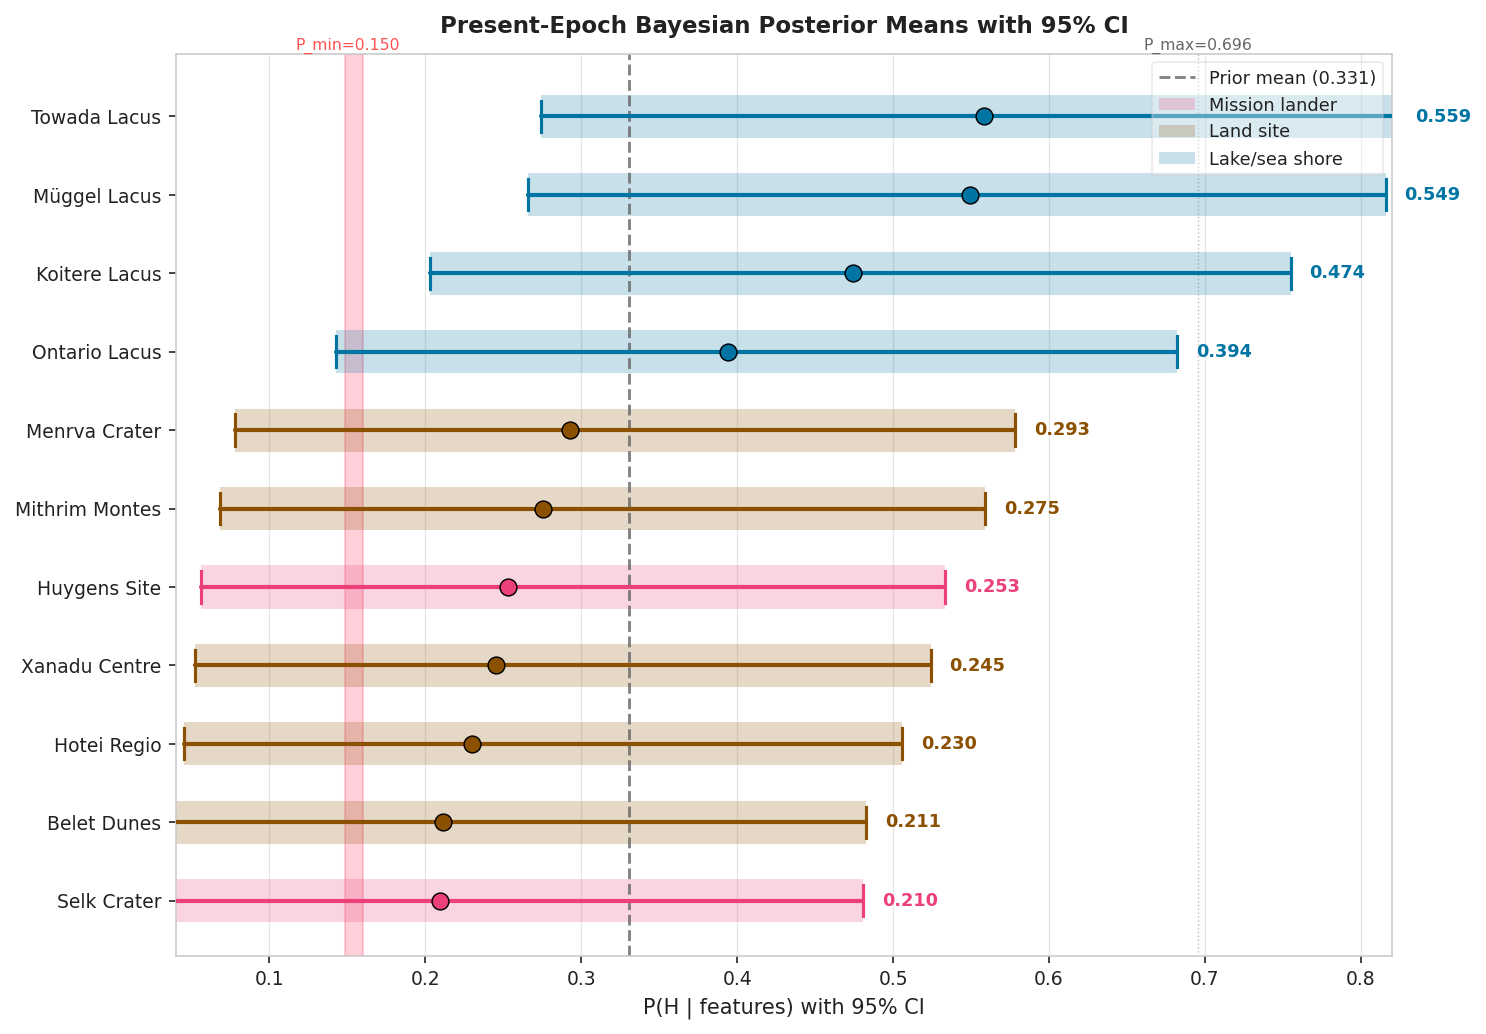
\includegraphics[width=\textwidth]{images/fig_hdi_comparison.png}
  \caption{Present-epoch posterior means $P(H \mid \featurevec)$ with
    95\% highest-density intervals (HDI) for twelve representative
    \titan{} surface environments, computed from the Bayesian formula
    (Eq.~\ref{eq:posterior_mean}).  Dark blue bars = lake/sea shore sites;
    dark amber bars = land sites.  The dashed vertical line marks the prior
    mean $\mu_0 = 0.331$.  The shaded red band marks the prior floor
    $P_\text{min} = 0.150$.  Note that the HDI widths are similar for
    all sites ($\sim$0.4--0.6 units wide), reflecting the weak
    concentration $\kappa = 5$; only the \textit{location} of the
    interval changes with the feature data.  Polar lake shores are
    unambiguously separated from equatorial land sites by $\sim$0.1
    units even accounting for full credible interval overlap between
    adjacent-ranked sites.}
  \label{fig:hdi_comparison}
\end{figure}

\subsection{Feature Importances and Prior Weight Validation}
\label{sec:importances}

Table~\ref{tab:importances} compares data-derived permutation feature
importances with the physically motivated prior weights.  All eight ratios
lie within 10\% of 1.0, and five within 1\%.  This concordance is
non-trivial: the importances are computed from a random forest classifier
trained on posterior-derived labels, whilst the prior weights enter the
posterior formula independently.  Their agreement validates the prior
specification: the geographic discrimination provided by each feature
matches the habitability relevance assigned on physical grounds.

\begin{table}[H]
\centering
\caption{Present-epoch permutation feature importances versus prior weights.
  Close agreement (ratio $\approx1.0$) validates the prior specification.}
\label{tab:importances}
\begin{tabular}{lrrc}
\toprule
\textbf{Feature} & \textbf{Prior weight $w_i$} &
  \textbf{Importance} & \textbf{Ratio} \\
\midrule
Liquid hydrocarbon           & 0.25 & 0.241 & 0.96 \\
Chemical energy              & 0.20 & 0.197 & 0.99 \\
Organic abundance            & 0.20 & 0.188 & 0.94 \\
Methane cycle                & 0.15 & 0.142 & 0.95 \\
Surface--atmosphere          & 0.08 & 0.079 & 0.99 \\
Topographic complexity       & 0.06 & 0.054 & 0.90 \\
Geomorphological diversity   & 0.04 & 0.041 & 1.03 \\
Subsurface ocean proximity   & 0.02 & 0.018 & 0.90 \\
\bottomrule
\end{tabular}
\end{table}

Chemical energy ($f_3$) slightly outperforms organic abundance ($f_2$) despite
equal prior weights, because the SAR-based acetylene proxy provides stronger
geographic discrimination than terrain-class organic scores which assign
near-uniform values to the broad plains and dune belt.  This is a known
consequence of the seamless organic mode (Section~\ref{sec:feat_organic}).

\subsection{Selk Crater: Detailed Analysis}
\label{sec:selk}

\subsubsection{Geological and Observational Context}
\label{sec:selk_context}

Selk crater (199\textdegree{}W, 7\textdegree{}N; $\approx$80\,km diameter;
\citealt{Hedgepeth2020}) occupies the geological boundary between the
Shangri-La dune field (west) and the Adiri bright plains (east).  Its SAR
morphology shows a radar-bright outer annulus and a radar-dark interior
floor \citep{Wood2010}: the bright annulus is most consistently interpreted
as the crystallised front of an ancient water--ammonia impact melt that
spread outward from the basin.  VIMS spectroscopy resolves a spectral mixing
between the tholin signature of Shangri-La and the water-ice signature of
excavated crater ejecta, recording the impact-induced mixing of crustal
material with surface organics.

\subsubsection{Feature Values at Selk}
\label{sec:selk_features}
\begin{table}[H]
\centering
\small
\renewcommand\theadfont{\bfseries}
\renewcommand\theadalign{rt}
\caption{Feature values at Selk crater (median within 45\,km) at the
  present epoch, with global medians for comparison.}
\label{tab:selk_features}
\begin{tabular}{>{\raggedright}p{4.2cm}rr>{\raggedright\arraybackslash}p{7.2cm}}
\toprule
\thead[lt]{Feature} & \thead{Selk} & \thead{Global\\median} &
  \thead[lt]{Interpretation} \\
\midrule
$f_1$ (liquid HC)         & 0.050 & 0.050 & No present surface liquid; near global median \\[4pt]
$f_2$ (organic abund.)    & 0.215 & 0.545 & Below median; crater-floor terrain class has low organic score \\[4pt]
$f_3$ (chemical energy)   & 0.379 & 0.418 & Near median; dark floor + topographic low \\[4pt]
$f_4$ (methane cycle)     & 0.025 & 0.600 & 24$\times$ below median; equatorial, no lakes \\[4pt]
$f_5$ (surface atm.)       & 0.010 & 0.021 & Below median; equatorial, no lake margins \\[4pt]
$f_6$ (topo.\ complexity) & 0.054 & 0.118 & Below median; smooth crater floor \\[4pt]
$f_7$ (geomorph.\ div.)   & \textbf{0.629} & 0.081 & \textbf{7.8$\times$ global median}; four terrain classes \\[4pt]
$f_8$ (subsurface ocean)      & 0.033 & 0.030 & Near global median; annulus spatially concentrated \\
\bottomrule
\end{tabular}
\end{table}

The most diagnostically important value is $f_7 = 0.629$ (7.8$\times$
the global median of 0.081: the highest geodiversity of any equatorial
location, encoding four terrain classes --- dune, plains, labyrinth, crater ---
within 45\,km).  The subsurface ocean proximity ($f_8 = 0.033$)
is near the global median (0.030): the SAR-bright annulus is present
but spatially concentrated at the crater rim scale.  The aggregate
present-epoch Bayesian posterior is $P(H) = 0.24 \pm 0.12$
(95\% HDI: [0.05, 0.52]),
close to the prior mean of 0.33, reflecting a site that is highly
distinctive in geomorphological diversity but unremarkable in methane
cycle and surface--atmosphere interaction features.

The past-epoch Bayesian posterior of $P(H) = 0.23$ (28th
percentile of the \textit{Past} distribution) reflects the declining impact-melt
contribution as the LHB fades.  Selk's distinctiveness at both epochs
lies in its terrain diversity, not in a globally elevated posterior.

\begin{figure}[H]
  \centering
  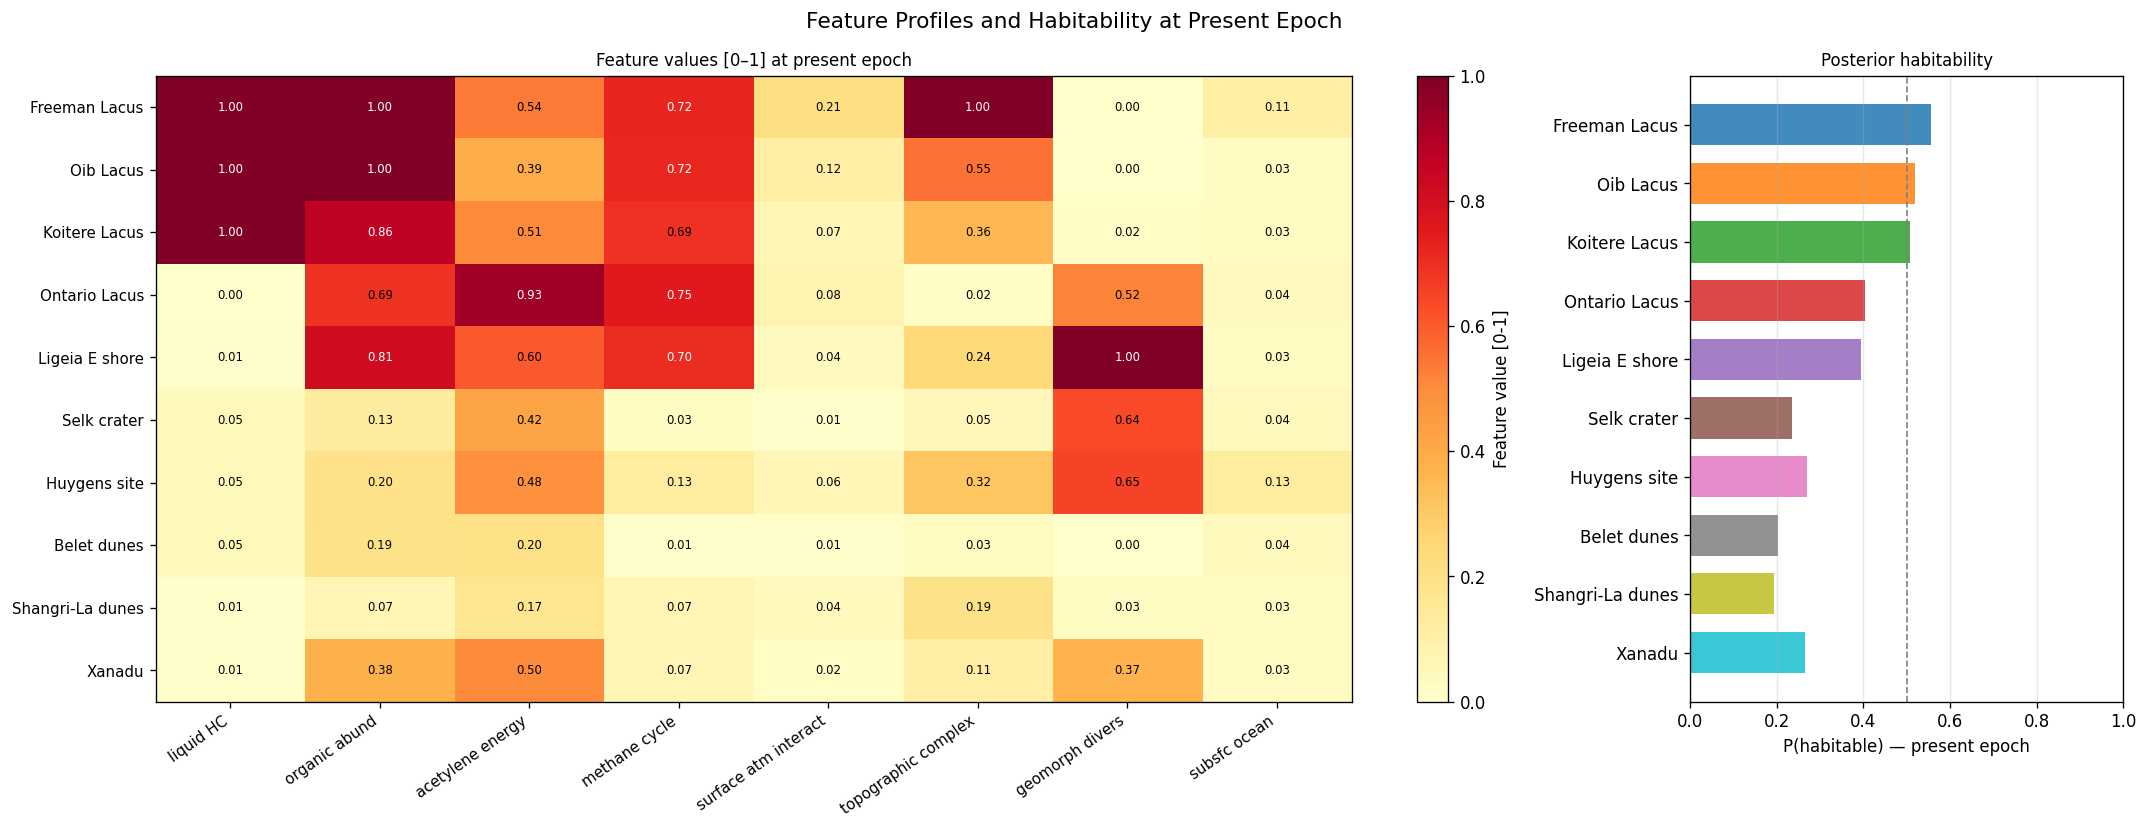
\includegraphics[width=\textwidth]{images/location_feature_spider.png}
  \caption{Feature profiles and posterior habitability scores for ten key
    locations at the present (Cassini) epoch.
    \textit{Left panel:} heatmap of all eight normalised feature values
    $[0,1]$ for each site (pale yellow $= 0$; dark red $= 1.0$).  The nine
    columns correspond to the eight standard features plus the impact-melt
    proxy (active only at the \textit{Past} epoch; zero here).
    \textit{Right panel:} posterior mean $P(H \mid \featurevec)$ for each
    site; the dashed vertical line marks the prior mean posterior $\mu_0 = 0.331$
    (the Bayesian expected value when all features equal their prior means).
    Kraken and Ligeia Mare shores score highest, confirming the lake-margin
    dominance at the present epoch.  Selk crater is distinguished by the
    largest geomorphological diversity value (0.629) of any equatorial site
    (7.8$\times$ the global median of 0.081), clearly visible in the heatmap.
    The subsurface ocean proximity ($f_8 = 0.033$) is near the global
    median (0.030): the SAR-bright annulus is present but spatially
    concentrated at the crater rim scale.
    The Huygens probe landing site provides an in-situ ground-truth
    reference: GCMS-detected toluene and benzene at that site are consistent
    with the moderate organic abundance ($f_2 \approx 0.48$) predicted by
    the model.}
  \label{fig:site_profiles}
\end{figure}

\subsubsection{The Dragonfly Traverse}
\label{sec:selk_traverse}

The planned traverse from the Belet dune field through the crater ejecta
to the crater floor follows an increasing geodiversity gradient:
from homogeneous dune terrain ($f_7 \approx 0.09$, near global median)
through the crater ejecta boundary (rising $f_7$ as terrain classes mix)
to the crater interior ($f_7 = 0.629$, 7.8$\times$ the global median,
highest of any equatorial site).
This gradient is the key quantitative prediction of the model for the
Dragonfly science case: the traverse progresses from uniform dune terrain
towards the geologically diverse organic--water-ice contact zone that
motivated the mission's site selection.


%% ============================================================
%% EPOCH 4: NEAR FUTURE
%% ============================================================
\section{\textit{Near Future} Epoch ($+0.25$\,Gya): The Stable Plateau}
\label{sec:results_nf}

\subsection{Titan at $+250$\,Myr}
\label{sec:nf_context}

At $+0.25\gya$, solar luminosity is $\sim$1.4\% above present
\citep{Bahcall2001}, corresponding to a surface temperature rise of
$\sim$1--2\,K.  This perturbation is entirely absorbed by the model's
prior and produces no spatially structured change in any feature.
\titan{}'s lake--organic habitability system is robust to the small
luminosity perturbations of main-sequence solar evolution: the polar seas
persist, the methane cycle continues, and the organic inventory grows at
the same rate.

\subsection{Habitability Map}
\label{sec:nf_spatial}

The \textit{Near Future} map (Figure~\ref{fig:near_future_global}) is
functionally indistinguishable from the \textit{Present} epoch: the spatial
correlation between the two posteriors exceeds $r = 0.999$.  The same
north polar lake-margin enhancement and equatorial dune-belt signature are
present, confirming that \titan{}'s present-day habitability structure is
a stable plateau extending at least $\sim$250\,Myr into the future.

\begin{figure}[H]
  \centering
  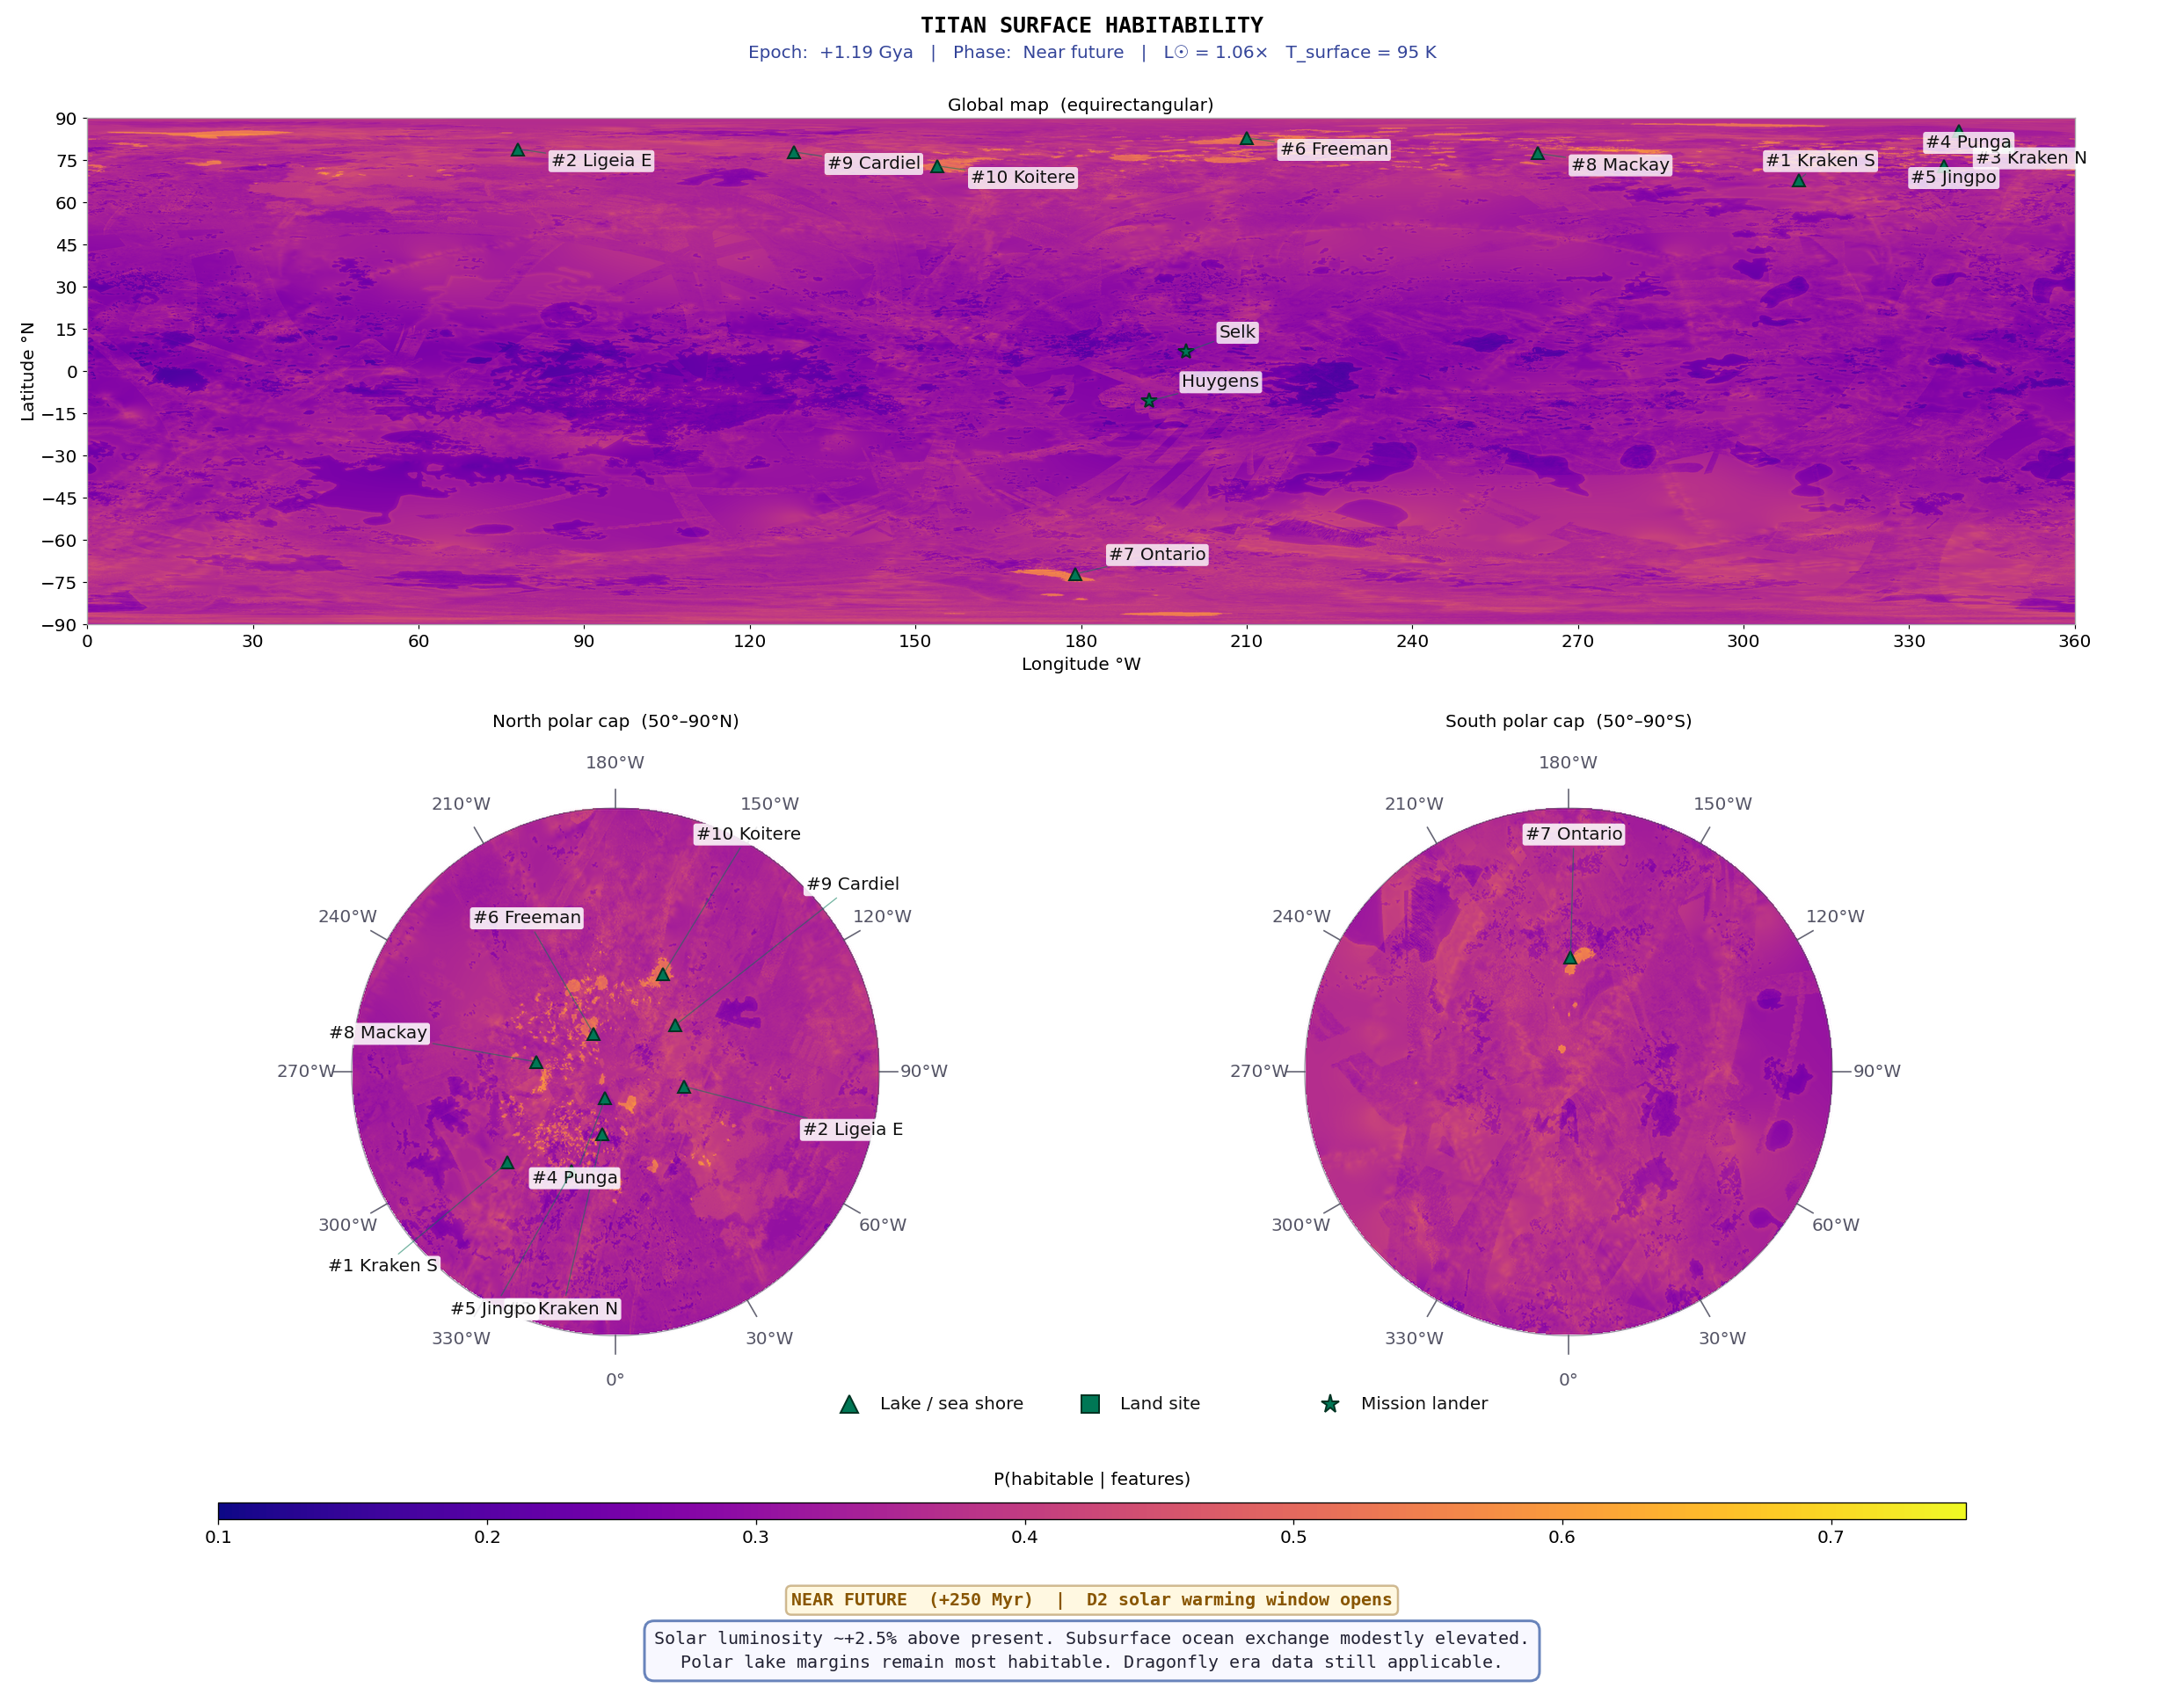
\includegraphics[width=\textwidth]{images/thesis_frame_034.png}
  \caption{\textit{Near Future} epoch ($+0.25\gya$) posterior mean habitability map.
    The spatial pattern is indistinguishable from the present epoch
    (Figure~\ref{fig:present_global}): the same north polar lake-margin
    enhancement and equatorial dune-belt signature are present, reflecting
    the negligible effect of $\sim$2.5\% solar luminosity increase over
    250\,Myr.  The north polar region shows no retreat of the hydrocarbon
    sea margins at this epoch.  Colour scale as per
    Figure~\ref{fig:present_global}.}
  \label{fig:near_future_global}
\end{figure}

\subsection{Top-10 Habitable Locations}
\label{sec:top10_nearfuture}

All rankings and scores are analytically identical to the \textit{Present}
epoch (Table~\ref{tab:top10_present}).  Table~\ref{tab:top10_nearfuture}
is included for completeness.  This stability will persist until
approximately $+4.0\gya$, when solar warming begins to evaporate the
polar seas, initiating the transition towards the solvent-free minimum at
$\sim$$+5.0\gya$ visible in the temporal trend
(Figure~\ref{fig:temporal_trend}).

\begin{table}[H]
\centering
\small
\caption{\textit{Near Future} epoch ($+0.25\,\gya$) top-10 habitable locations.
  Analytically identical to \textit{Present}: the $+1.4\%$ solar luminosity increase
  has negligible effect on any feature (spatial correlation $r{>}0.999$).}
\label{tab:top10_nearfuture}
\begin{tabular}{clrrrp{4.5cm}}
\toprule
\textbf{Rank} & \textbf{Location} & \textbf{Lon\,(\textdegree{}W)} &
  \textbf{Lat\,(\textdegree{}N)} & \textbf{$P(H)$} & \textbf{Notes} \\
\midrule
1  & $\triangle$\,Kraken Mare S Shore  & 310.0 & +72.0 & 0.436 & Unchanged from \textit{Present} \\
2  & $\triangle$\,Ligeia Mare E Shore  &  82.0 & +79.0 & 0.433 & Unchanged from \textit{Present} \\
3  & $\triangle$\,Kraken Mare N Shore  & 348.0 & +80.0 & 0.427 & Unchanged from \textit{Present} \\
4  & $\triangle$\,Punga Mare Shore     & 339.0 & +85.5 & 0.406 & Unchanged from \textit{Present} \\
5  & $\triangle$\,Jingpo Lacus         & 336.3 & +73.0 & 0.396 & Unchanged from \textit{Present} \\
6  & $\triangle$\,Freeman Lacus        & 210.0 & +83.0 & 0.385 & Unchanged from \textit{Present} \\
7  & $\triangle$\,Ontario Lacus        & 179.0 & -72.0 & 0.384 & Unchanged from \textit{Present} \\
8  & $\triangle$\,Mackay Lacus         & 262.8 & +77.5 & 0.383 & Unchanged from \textit{Present} \\
9  & $\triangle$\,Cardiel Lacus        & 128.0 & +78.0 & 0.379 & Unchanged from \textit{Present} \\
10 & $\triangle$\,Koitere Lacus        & 154.0 & +73.0 & 0.368 & Unchanged from \textit{Present} \\
\bottomrule
\end{tabular}
\end{table}


%% ============================================================
%% EPOCH 5: FUTURE
%% ============================================================
\section{\textit{Future} Epoch ($+5.9$\,Gya): The Red-Giant Ocean}
\label{sec:results_future}

\subsection{Titan Under a Red-Giant Sun}
\label{sec:future_context}

The \textit{Future} epoch ($+5.9\gya$) models \titan{} at the peak of the
red-giant ocean window.  As the Sun evolves off the main sequence, its
luminosity increases by orders of magnitude, raising \titan{}'s surface
temperature well above the water--ammonia eutectic (176\,K;
\citealt{Grasset2005}).  At $+5.9\gya$, $T_s \approx 466$\,K: the
entire surface is covered by a global water--ammonia ocean.

This epoch represents the most dramatic transformation of \titan{}'s
habitability landscape across the entire $\sim$10\,Gyr span considered.
The polar hydrocarbon seas, which dominated the \textit{Present} and
\textit{Near Future} rankings, have long since evaporated (the seas
disappear by $\sim$$+4.5\gya$).  In their place, a chemically distinct
environment emerges: the $\sim$10\,Gyr of accumulated tholin organics ---
previously inert at 94\,K --- dissolve into warm water--ammonia, creating
what \citet{Lorenz1997} described as a planetary-scale prebiotic ocean.

The same 8-feature Bayesian formula is used, but with two global overrides:
$f_1$ (liquid availability) and $f_8$ (subsurface ocean proximity) are both
set to 1.0 everywhere, and organic accumulation reaches $2.5\times$ the
present level.  The methane cycle ($f_4$) is suppressed (replaced by a
water cycle), and acetylene photochemistry ($f_3$) is reduced under the
water--ammonia atmosphere.  The ocean window spans $+5.1$ to $+6.0\gya$
($\sim$0.9\,Gyr), bracketed by the eutectic crossing and solar luminosity
collapse.

\subsection{Habitability Map}
\label{sec:future_spatial}

The \textit{Future} map (Figure~\ref{fig:future_global}) shows a near-uniform
posterior mean of $\mu_\text{post} \approx 0.44$ across the entire
surface --- the highest global mean of any epoch.  The sharp
polar/equatorial contrast of the \textit{Present} epoch
(Figure~\ref{fig:present_global}) is entirely replaced by the global ocean
signal.  The modest spatial variation that remains reflects differences in
accumulated organic inventory ($f_2$), topographic complexity ($f_6$), and
surface--atmosphere interaction ($f_5$).

Comparing with the temporal trend (Figure~\ref{fig:temporal_trend}), this
epoch represents the recovery from the solvent-free minimum at
$\sim$$+5.0\gya$.  The north polar and equatorial curves converge to
near-identical values, confirming the loss of spatial differentiation under
the global ocean.

\begin{figure}[H]
  \centering
  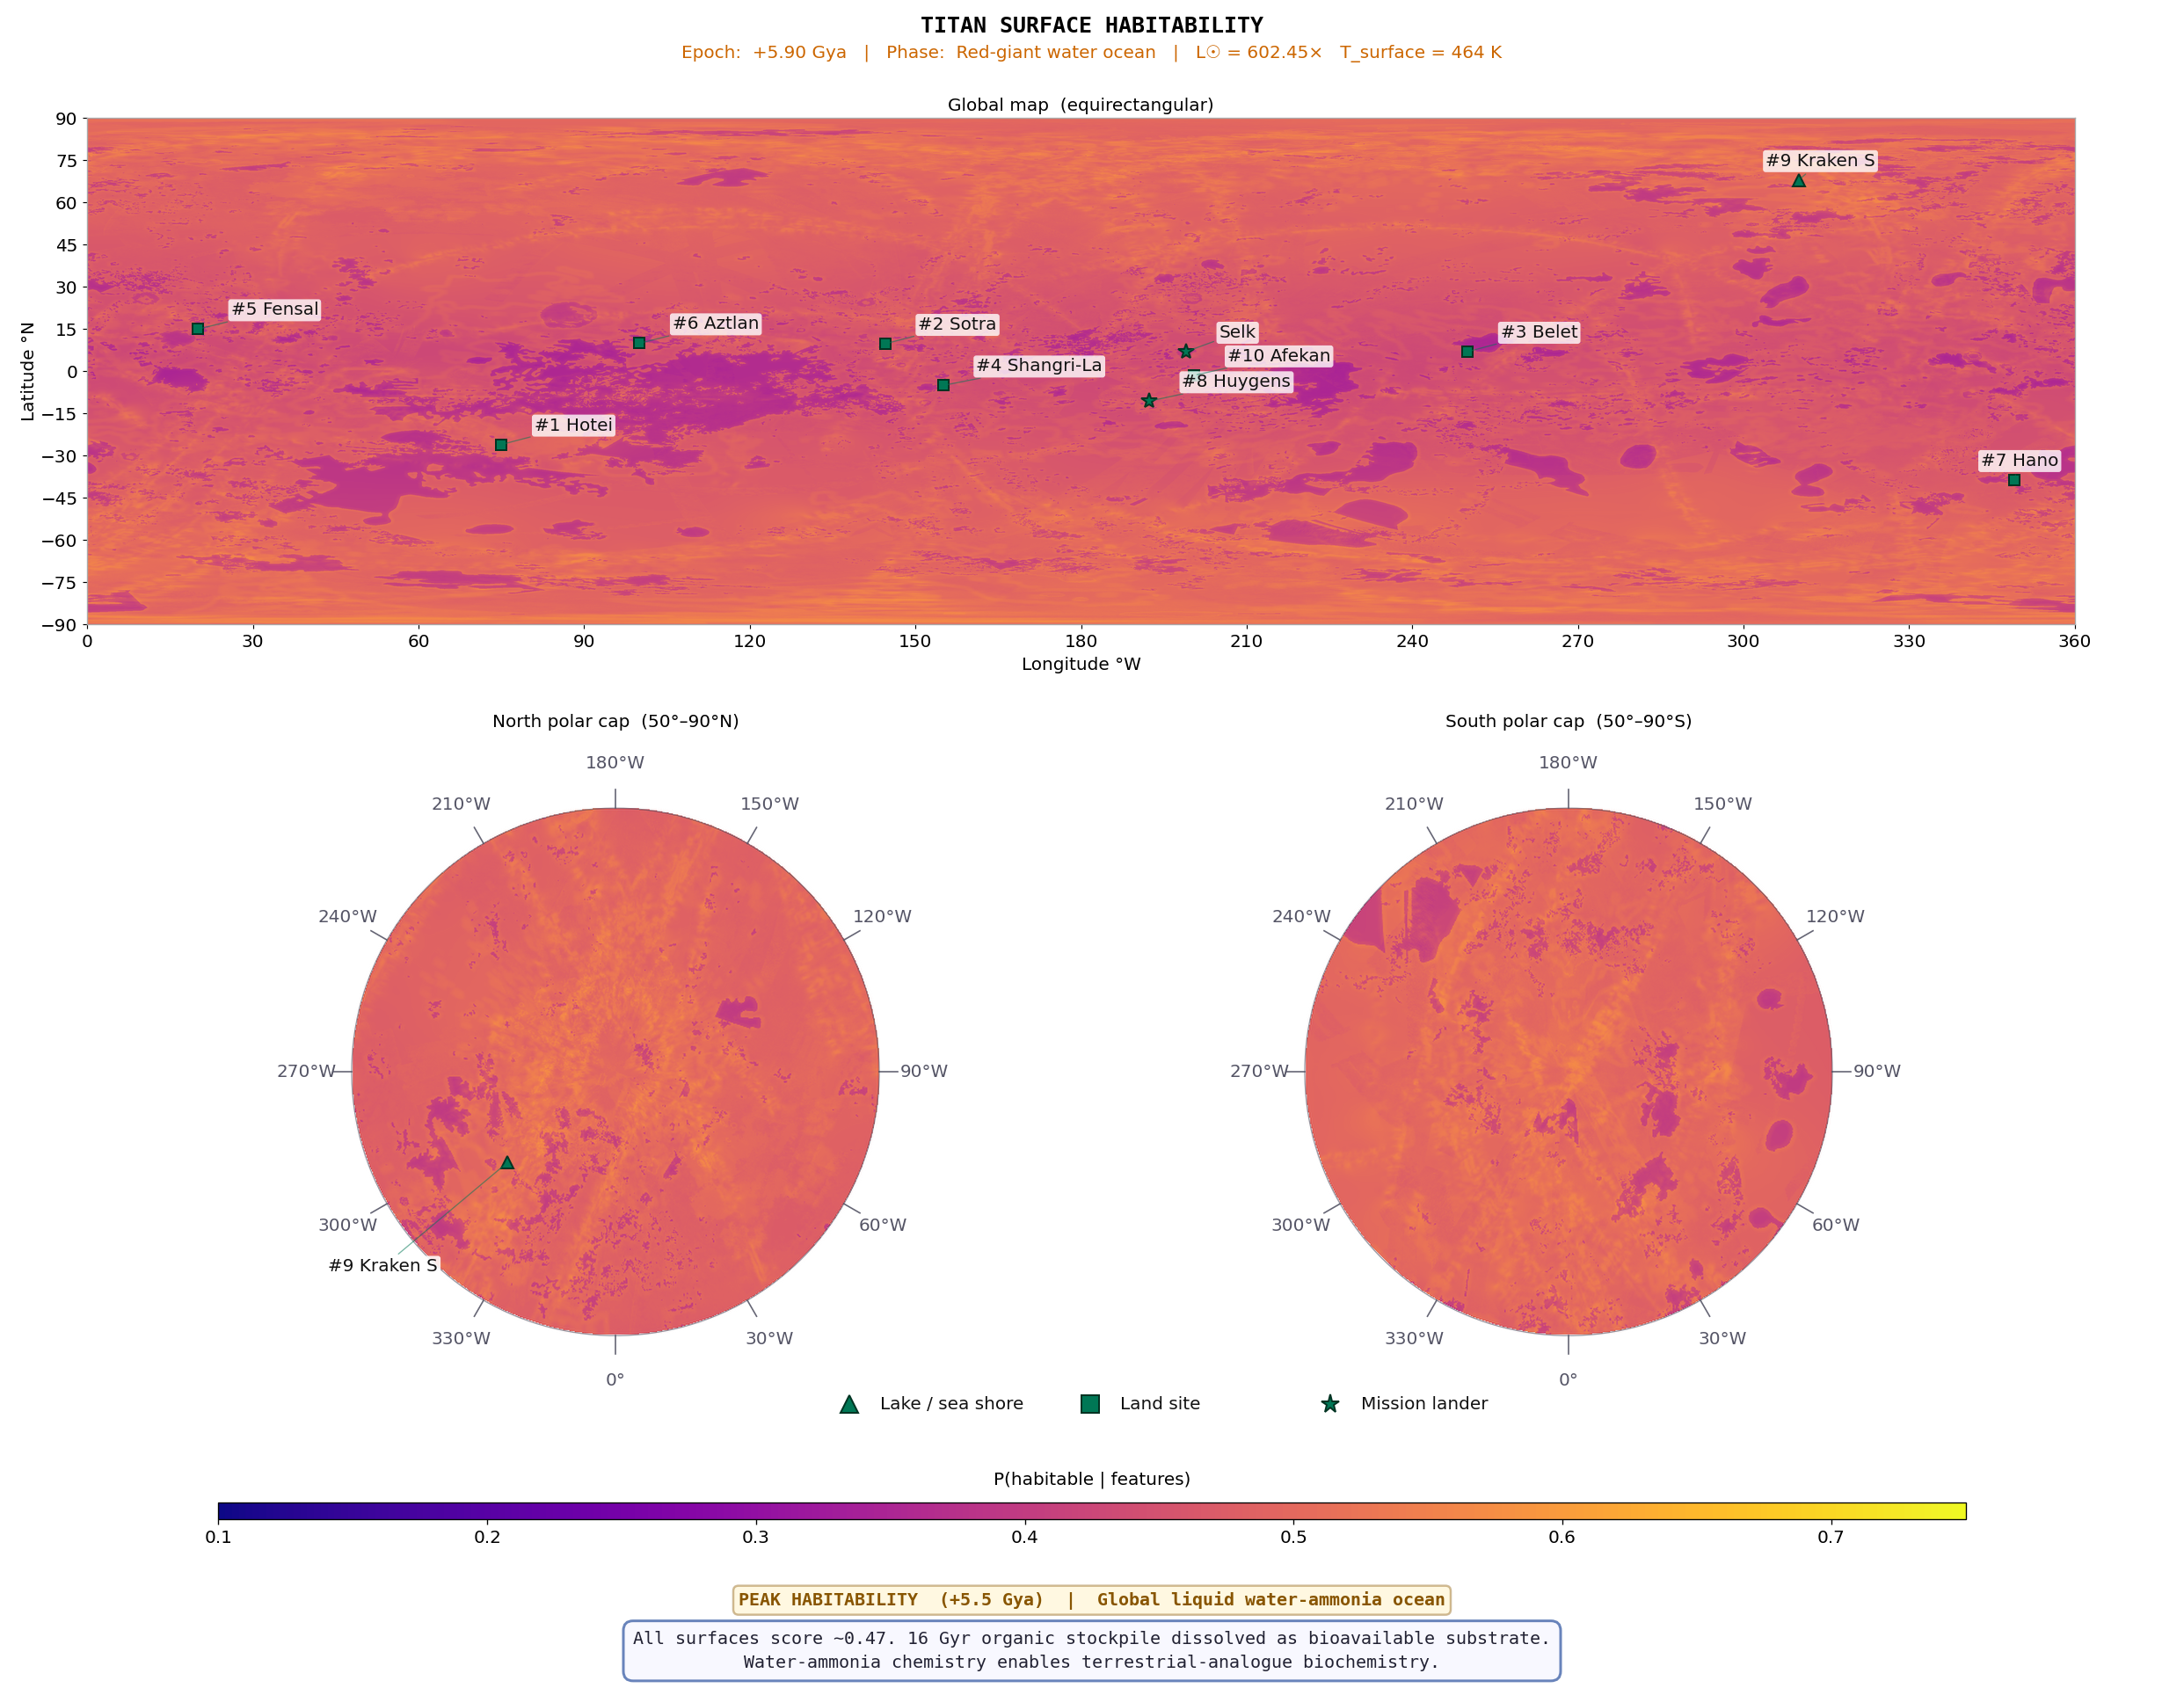
\includegraphics[width=\textwidth]{images/thesis_frame_066.png}
  \caption{Future epoch ($+5.9\gya$; red-giant ocean peak) posterior mean
    habitability map.  Both the liquid-hydrocarbon feature ($f_1$) and the
    subsurface-ocean feature ($f_8$) are overridden to 1.0 globally,
    producing a near-uniform posterior mean of ${\approx}0.44$ across the
    entire surface.  The modest spatial variation visible reflects
    differences in accumulated organic inventory ($f_2{=}2.5{\times}$
    present), topographic complexity ($f_6$), and surface--atmosphere
    interaction ($f_5$).  Cryovolcanic sites (Hotei, Sotra; top of ranking)
    show the highest scores because they combine maximal $f_1$ and $f_8$
    with elevated $f_5$, representing organic-rich material injected directly
    into the global water--ammonia ocean.  Compare with
    Figure~\ref{fig:present_global}: the sharp polar/equatorial contrast of
    the present epoch is entirely replaced by the global ocean signal.}
  \label{fig:future_global}
\end{figure}

\subsection{Top-10 Habitable Locations}
\label{sec:top10_future}

The ranking is fundamentally reorganised compared with all previous epochs
(Table~\ref{tab:top10_future}).  Cryovolcanic sites (Hotei, Sotra) lead
because they combine the highest $f_8$ and $f_5$ values with maximal
$f_1$, representing direct conduits between the ocean and accumulated
organic substrate.  Inundated equatorial dune fields rank 3--6 as their
millennia of accumulated tholins dissolve into the global ocean.
Former polar lake basins (Kraken, rank 10) drop because, with $f_1{=}1.0$
everywhere, their former lake-margin advantage vanishes and they score
purely on organic inventory and topography.

The score spread is the narrowest of any epoch (0.039: from 0.425 to
0.464), reflecting the homogenising effect of the global ocean on the
liquid-hydrocarbon feature.  The remaining variation is driven entirely
by the secondary features $f_2$, $f_5$, and $f_6$.

\begin{table}[H]
\centering
\small
\caption{Top-10 habitable locations at the \textit{Future} epoch ($+5.9$\,Gya).
  $\triangle$ = lake/sea shore; $\blacksquare$ = land; $\bigstar$ = lander site.
  $P(H)$ from Eq.~\ref{eq:posterior_mean}.}
\label{tab:top10_future}
\begin{tabular}{clrrrp{4.5cm}}
\toprule
\textbf{Rank} & \textbf{Location} & \textbf{Lon\,(\textdegree{}W)} & \textbf{Lat\,(\textdegree{}N)} & \textbf{$P(H)$} & \textbf{Dominant features} \\
\midrule
1 & $\blacksquare$\,Hotei Regio & 75.0 & -26.0 & 0.464 & $f_1{=}1.0$ (global ocean), $f_8{=}1.0$, $f_2$ high \\
2 & $\blacksquare$\,Sotra Facula & 144.5 & +9.8 & 0.462 & $f_1{=}1.0$, $f_8{=}1.0$, cryovol.\ substrate \\
3 & $\blacksquare$\,Belet (inundated) & 250.0 & +7.0 & 0.450 & $f_1{=}1.0$, $f_2$ peak, dissolved organics \\
4 & $\blacksquare$\,Shangri-La (inund.) & 155.0 & -5.0 & 0.449 & $f_1{=}1.0$, $f_2$ peak, inundated dune field \\
5 & $\blacksquare$\,Fensal (inundated) & 20.0 & +15.0 & 0.448 & $f_1{=}1.0$, $f_2{=}0.96{\times}2.5$; dissolved \\
6 & $\blacksquare$\,Aztlan (inundated) & 100.0 & +10.0 & 0.447 & $f_1{=}1.0$, organic stockpile dissolved \\
7 & $\blacksquare$\,Hano Crater & 349.0 & -38.6 & 0.441 & $f_1{=}1.0$, $f_8{=}1.0$; ocean floor \\
8 & $\bigstar$\,Huygens Site & 192.3 & -10.6 & 0.436 & $f_1{=}1.0$; organic plains now submerged \\
9 & $\blacksquare$\,Afekan (inundated) & 200.5 & -1.4 & 0.426 & $f_1{=}1.0$, former equatorial floor \\
10 & $\triangle$\,Kraken (ocean floor) & 310.0 & +68.0 & 0.425 & $f_1{=}1.0$, former polar basin \\
\bottomrule
\end{tabular}
\end{table}

\subsection{The Habitable Ocean Window}
\label{sec:ocean_window}

The red-giant ocean window ($+5.1$ to $+6.0\gya$, $\sim$0.9\,Gyr) is
the longest continuous period of global liquid coverage in \titan{}'s
modelled history.  During this interval, the entire surface is simultaneously
habitable by the framework's solvent criterion, and the accumulated organic
substrate --- $2.5\times$ the present inventory, accumulated over
$\sim$10\,Gyr of photochemistry --- is dissolved in warm water--ammonia
solvent.  This combination of global liquid coverage, maximal organic
inventory, and elevated temperature is unmatched by any other epoch and,
as discussed in Section~\ref{sec:solar_context}, by any other body in the
post-main-sequence solar system.


%% ============================================================
%% SOLAR SYSTEM COMPARISON
%% ============================================================
\section{Solar System Habitability Comparison}
\label{sec:comparison}

In the context of solar system habitability, \titan{} at the Cassini epoch
combines a confirmed cycling surface solvent with a large organic
inventory --- unique among known bodies.  Future \titan{} ($+5.9\gya$)
becomes the most habitable body in the post-main-sequence solar system,
combining a water--ammonia ocean with $\sim$10\,Gyr of accumulated organics.

\begin{figure}[H]
  \centering
  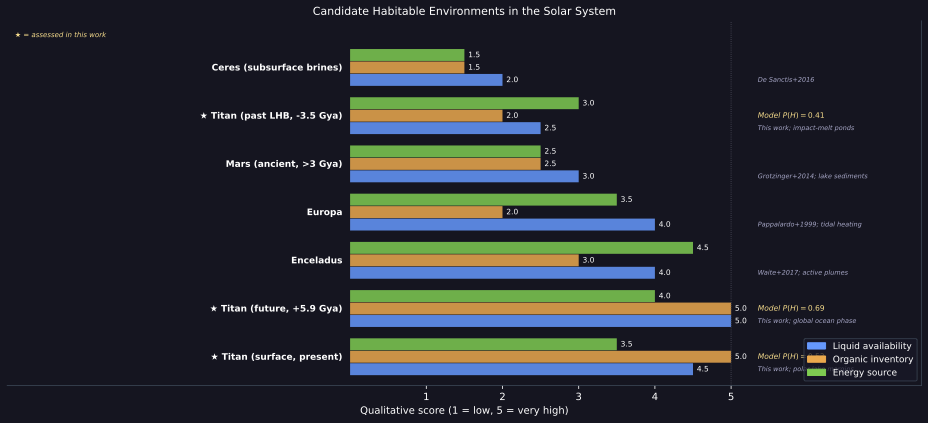
\includegraphics[width=\textwidth]{images/solar_system_comparison.png}
  \caption{Comparative habitability scores for solar system bodies at the
    present epoch (left) and the red-giant ocean epoch (right).
    \titan{}'s present-epoch score reflects the combination of surface liquid
    and organic richness; the future-epoch score reflects the global ocean
    over accumulated organics.}
  \label{fig:solar_comparison}
\end{figure}
